\documentclass{article}
\usepackage{amsmath}    % For mathematical symbols
\usepackage{booktabs}   % For professional table formatting
\usepackage{tabularx}   % For flexible tables
\usepackage{xcolor}     % For row colors
\usepackage{array}      % For flexible column formatting
\usepackage{graphicx}   % For including logos or images
\usepackage[a4paper, top=1in, bottom=1in, left=0.8in, right=0.8in]{geometry}
\usepackage{lipsum}   % For placeholder text
\usepackage{caption}
\usepackage{subcaption}
\usepackage{hyperref}


\setlength{\parskip}{1em}  % Adds 1em of vertical space between paragraphs

\begin{document}

% Title
\title{Foundations and Frontiers of Machine Learning\\Group Assignment 2\\Group 1}
\author{}
\date{}
\maketitle

% Table of Contents
\tableofcontents
\newpage

% Lists
\listoffigures
\listoftables
\newpage

% Sections
\section{Table of Contributions}

\begin{table}[h!]
    \centering
    \begin{tabular}{|l|l|l|}
        \hline
        \textbf{Name} & \textbf{Student ID} & \textbf{Contribution} \\ \hline
        Emmanouil Tsolias       & 239490757 & Task 1 \\ \hline
        Emmanouil Tsolias       & 239490757 & Task 2 \\ \hline
        Emmanouil Tsolias       & 239490757 & Task 3 \\ \hline
        Emmanouil Tsolias       & 239490757 & Task 4 \\ \hline
        Emmanouil Tsolias       & 239490757 & Task 5 \\ \hline
        -       & - & Task 6 \\ \hline
    \end{tabular}
    \caption{Individual Contribution to Group Work}
    \label{tab:contributions}
\end{table}
\newpage

\section{Data Visualisation (Task 2)}
\subsection{Visualing with PCA}

Machine learning models use data to finetune the values of their internal parameters while training.
Bigger datasets can contain more information but sometimes multiple features contain the same information scaled.
This becomes more likely with larger datasets.
Moreover, each additional feature adds a new dimension to the dataset which makes the samples sparse, and visualisation harder. (Khee, 2022).

This can be addressed by constructing new features that encompass the dataset’s information without repetition, using with the Principal Components Analysis (PCA) technique.
The first new feature is engineered to explain as much variance as possible from all features of the dataset (Maćkiewicz, 1993).
Each next one is engineered to contain as much of the information that is left, without repetition, which means that the last features contain little to no additional information (depending on how linearly independent the dataset was) and can be discarded, allowing for easier visualization and reducing the overall noise.
Also, the features are now in descending order in terms of variance explained so we can select the first n ones, knowing that we have retain maximum information per feature.
We can now select a number that is suitable for visualization.
The new features have no actual meaning but can be used to show the distribution of the samples in the space, informing us about the separability of the classes.

\begin{figure}[h!]
    \centering
    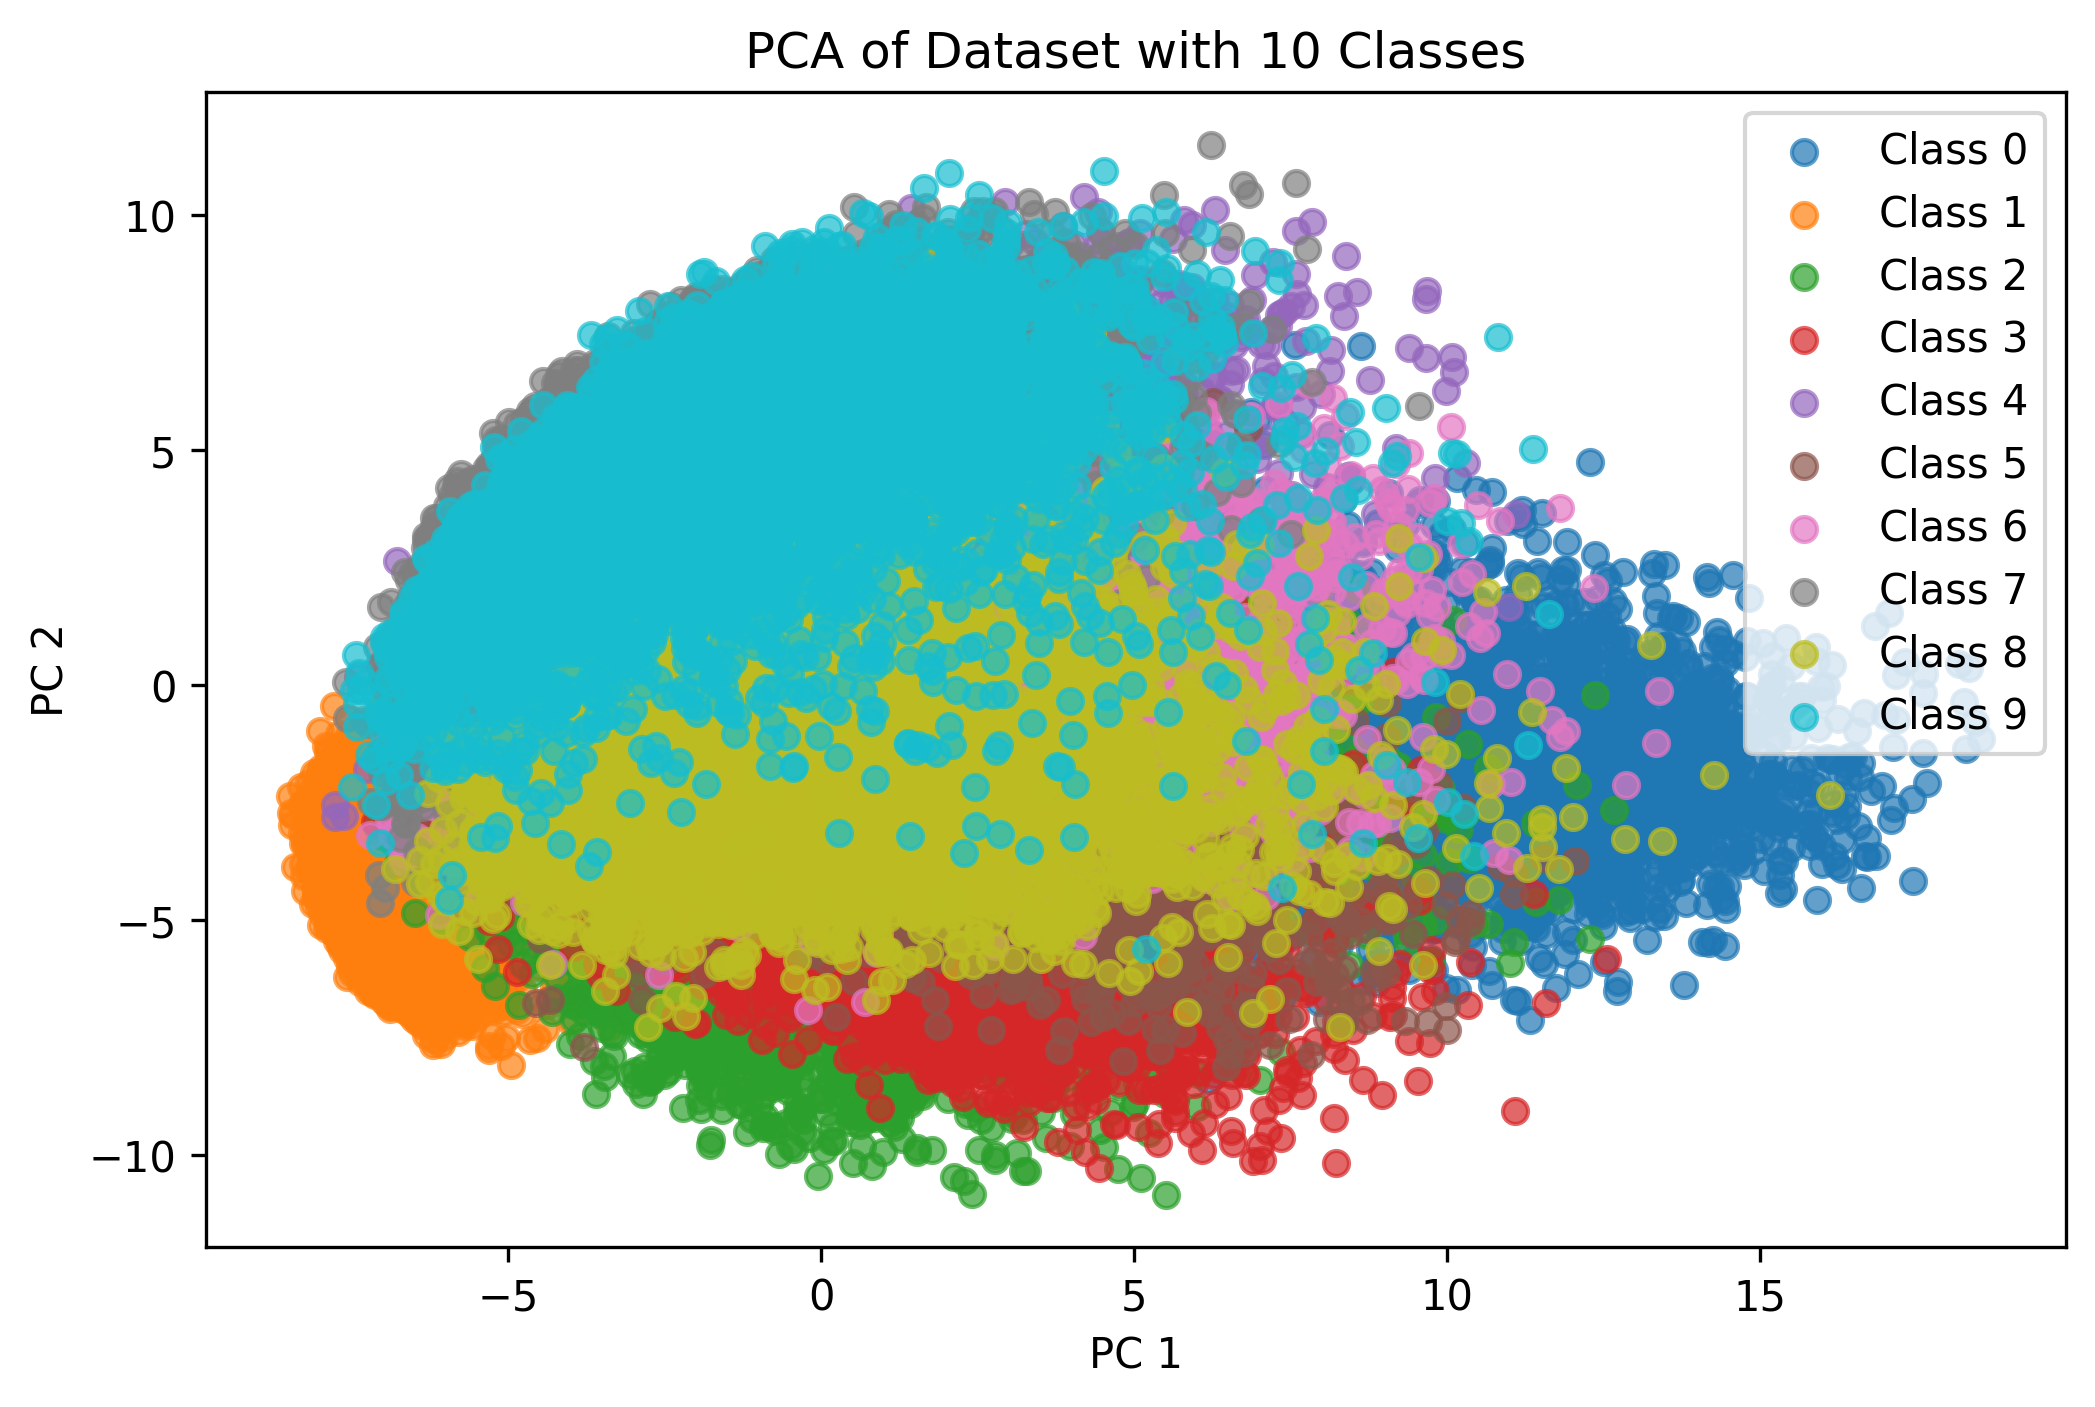
\includegraphics[width=0.5\textwidth]{./plots/plot1.png}
    \caption{Plot of 2 first components of PCA for all digits of the MNIST dataset.}
    \label{fig:plot1}
\end{figure}

If we plot the first two components with different colour for each class, we can see which classes overlap, and which ones are linearly separable.
Thus we have that, for example, the pairs (0, 1), (0, 2), and (2, 9) should be easy to differentiate since the occupy opposing parts on the plane.
Still, due to the significant overlap caused by 10 different classes, the distribution of some of the classes is obscured. 

\begin{figure}[h!]
    \centering
    \begin{subfigure}[t]{0.45\textwidth}
        \centering
        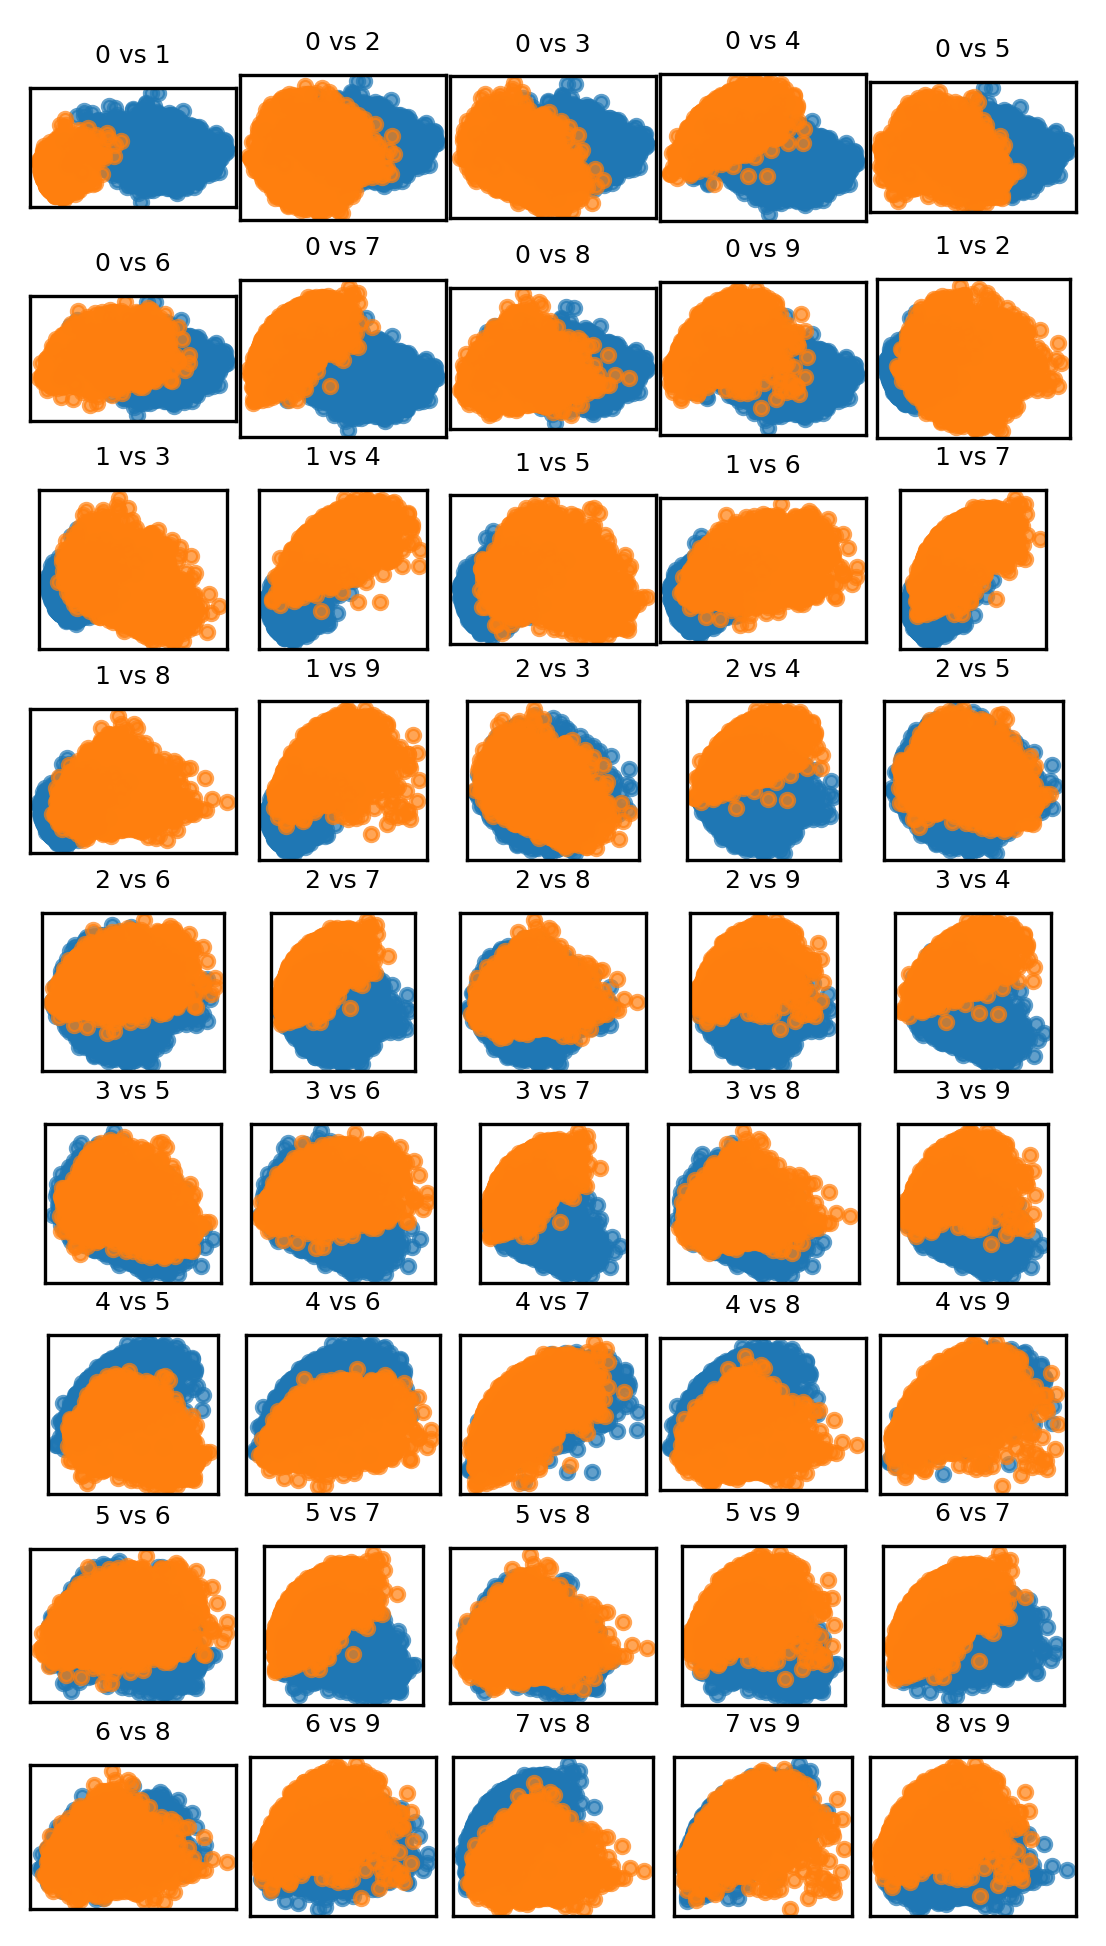
\includegraphics[width=\textwidth]{./plots/plot2.png}
        \caption{Plot of the first 2 PCA Components for all pairs of digits.}
        \label{fig:plot2a}
    \end{subfigure}
    \hspace{0.02\textwidth}
    \begin{subfigure}[t]{0.45\textwidth}
        \centering
        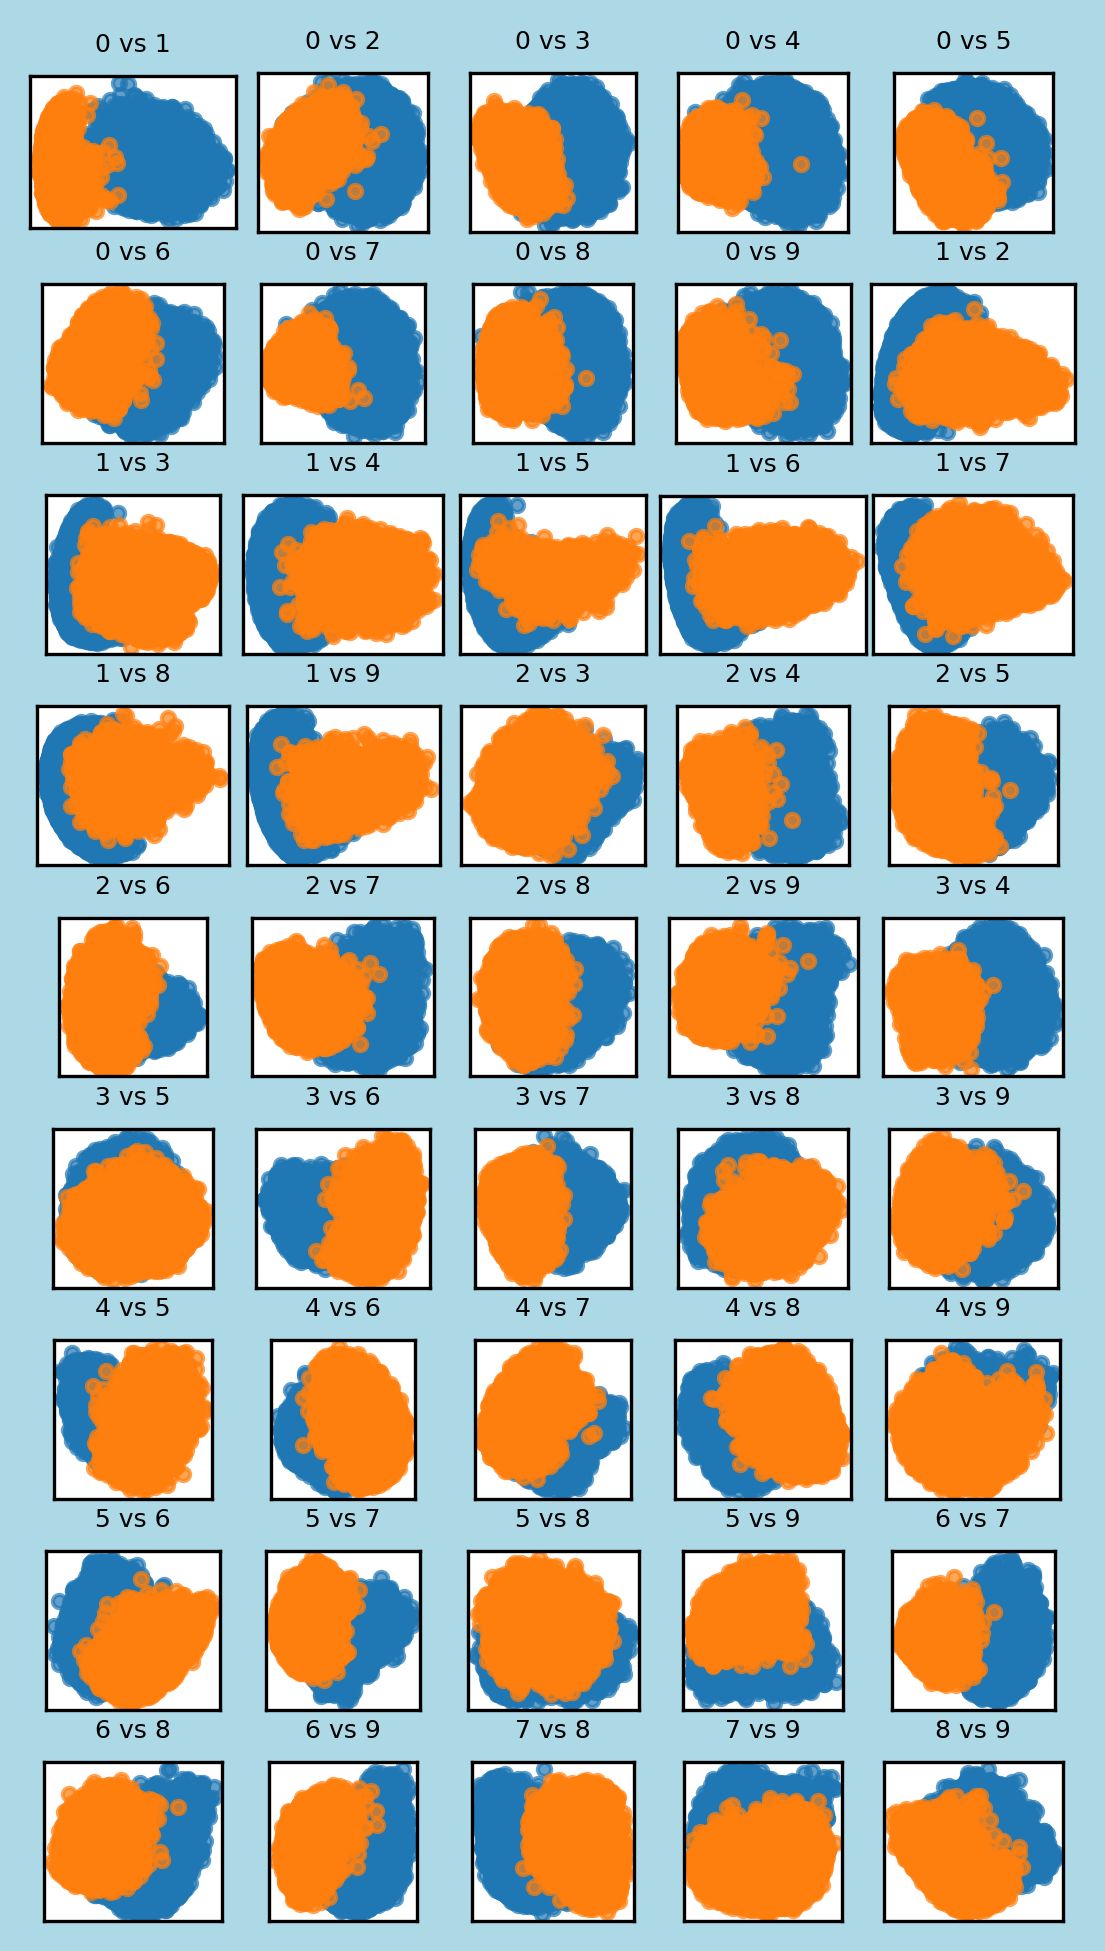
\includegraphics[width=\textwidth]{./plots/plot3.png}
        \caption{Pair-wise PCA plot.}
        \label{fig:plot2b}
    \end{subfigure}
    \caption{Side-by-side visualization of PCA components and pair-wise PCA plots.}
    \label{fig:side_by_side}
\end{figure}

Figure 2a provides a pairwise visualisation of the distributions.
It Is clear that some pairs of classes, e.g. (0, 1), (0, 7), (3, 7) are relatively distinct, while others (5, 8), (7, 9) are virtually impossible to separate.
However this is the result of considering just 2 components and not all of the information contained in the dataset.
That means distributions that do not seem differentiable now, may actually be when the model is trained on the original dataset.
Another point is that the above results are obtained by performing PCA on the whole dataset.
However, when it comes to distinguishing classes in pairs, the datapoints of other classes introduce variance and noise that may be irrelevant.
Thus, it is worth producing the same plot with the PCA calculated for each pair.
This is shown in figure 2b and it becomes apparent that the results are better in terms of separability.
To objectively measure this, we use the silhouette score which takes into account the average distance of a clusters samples between each-other and between the samples of the other class (Shahpure, 2020).
Higher scores mean better clustering and for the generic PCA we get 0.337 where as the same score for the pairwise PCA is 0.407.
This proves that we can achieve better clustering (and hence prediction performance) by performing pairwise PCA.


\subsection{Mathematical basis of PCA}
Before applying and transformations on the dataset, it is important to normalize it so the features with larger ranges do not affect the calculations disproportionately. 

\begin{figure}[h!]
    \centering
    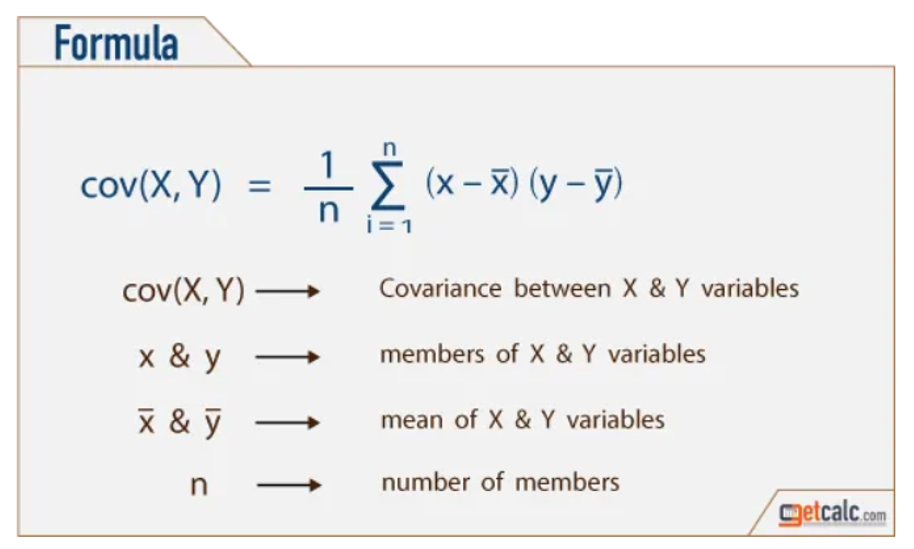
\includegraphics[width=0.5\textwidth]{./plots/plot4.png}
    \caption{Calculation of Covariance Matrix (Dubey, 2018).}
    \label{fig:plot3}
\end{figure}

The next step is to identify how much each feature correlates with the other ones, as the more they correlate, the less useful information they add.
Figure 4 shows the steps of calculation, which essentially shows that the more two variables follow the same trend, then larger the product of their difference to the mean will be

From Linear Algebra we know that a matrix can represent a transformation and its eigenvectors represent the directions in which the data has the most variance.
Thus these eigenvectors will form the basis of the new vector space which is now built so that each new dimensions contains the most variance

The actual amount of variance explained by each dimension is given away by the eigenvalues of the eigenvectors.
We can create a new matrix by concatenating the desired number of eigenvectors which, when multiplied with our data, produces the PCA-Data, which is our data transformed to the new base. 

\section{Perceptrons (Task 2)}

The human neurons receive multiple stimulations that are then regulated (scaled).
The result then is not a linear stimulation but instead a binary state of excitation, equivalent to “making a decision” (Queensland Brain Institute).
Rosenblatt’s perceptron machine is a software analogous which receives a multidimensional input that it individually scales, and then compares its sum to a bias in order to select a binary response (Rosenblatt, 1958).
If the input is the coordinates of some samples the classes of which are known, we can calculate the weights and the bias, which are trainable parameters, to produce the desired response.
Since the described operation is the equation of the line or a hyperplane, we can set up an algorithm that hypotheses which plane would separate these classes based on the values of their coordinates, and if this hypothesis is wrong, it changes it so that it would work well for these specific samples.
If the samples occupy distinct areas of the feature space and we do that for all samples, the resulting hyperplane would end up satisfying the requirement for all samples (since we know the samples of a cluster have similar feature values) (Rosenblatt, 1958).
From Task 1 we know that this applies to a degree, for the digit pairs.

The algorithmic approach consists of two functions.
The first implements the matrix multiplication/scaling and the comparison with the threshold to return a result/decision.
The second iterates through the samples of the dataset, producing a prediction and then correcting the weights so that if the prediction was wrong, next time it will be closer to right.
The algorithms stops upon achieving an MSE goal or reaching the iterations threshold.
With each iteration the number of misclassifications reduces on the training dataset, but the same is not always true for the test dataset, as the two contain different samples and too accurate a modeling of the training samples can end up imprinting noise on the model (overfitting).
This is demonstrated by the training vs test accuracy, over number of iterations in figure 4.

\begin{figure}[h!]
    \centering
    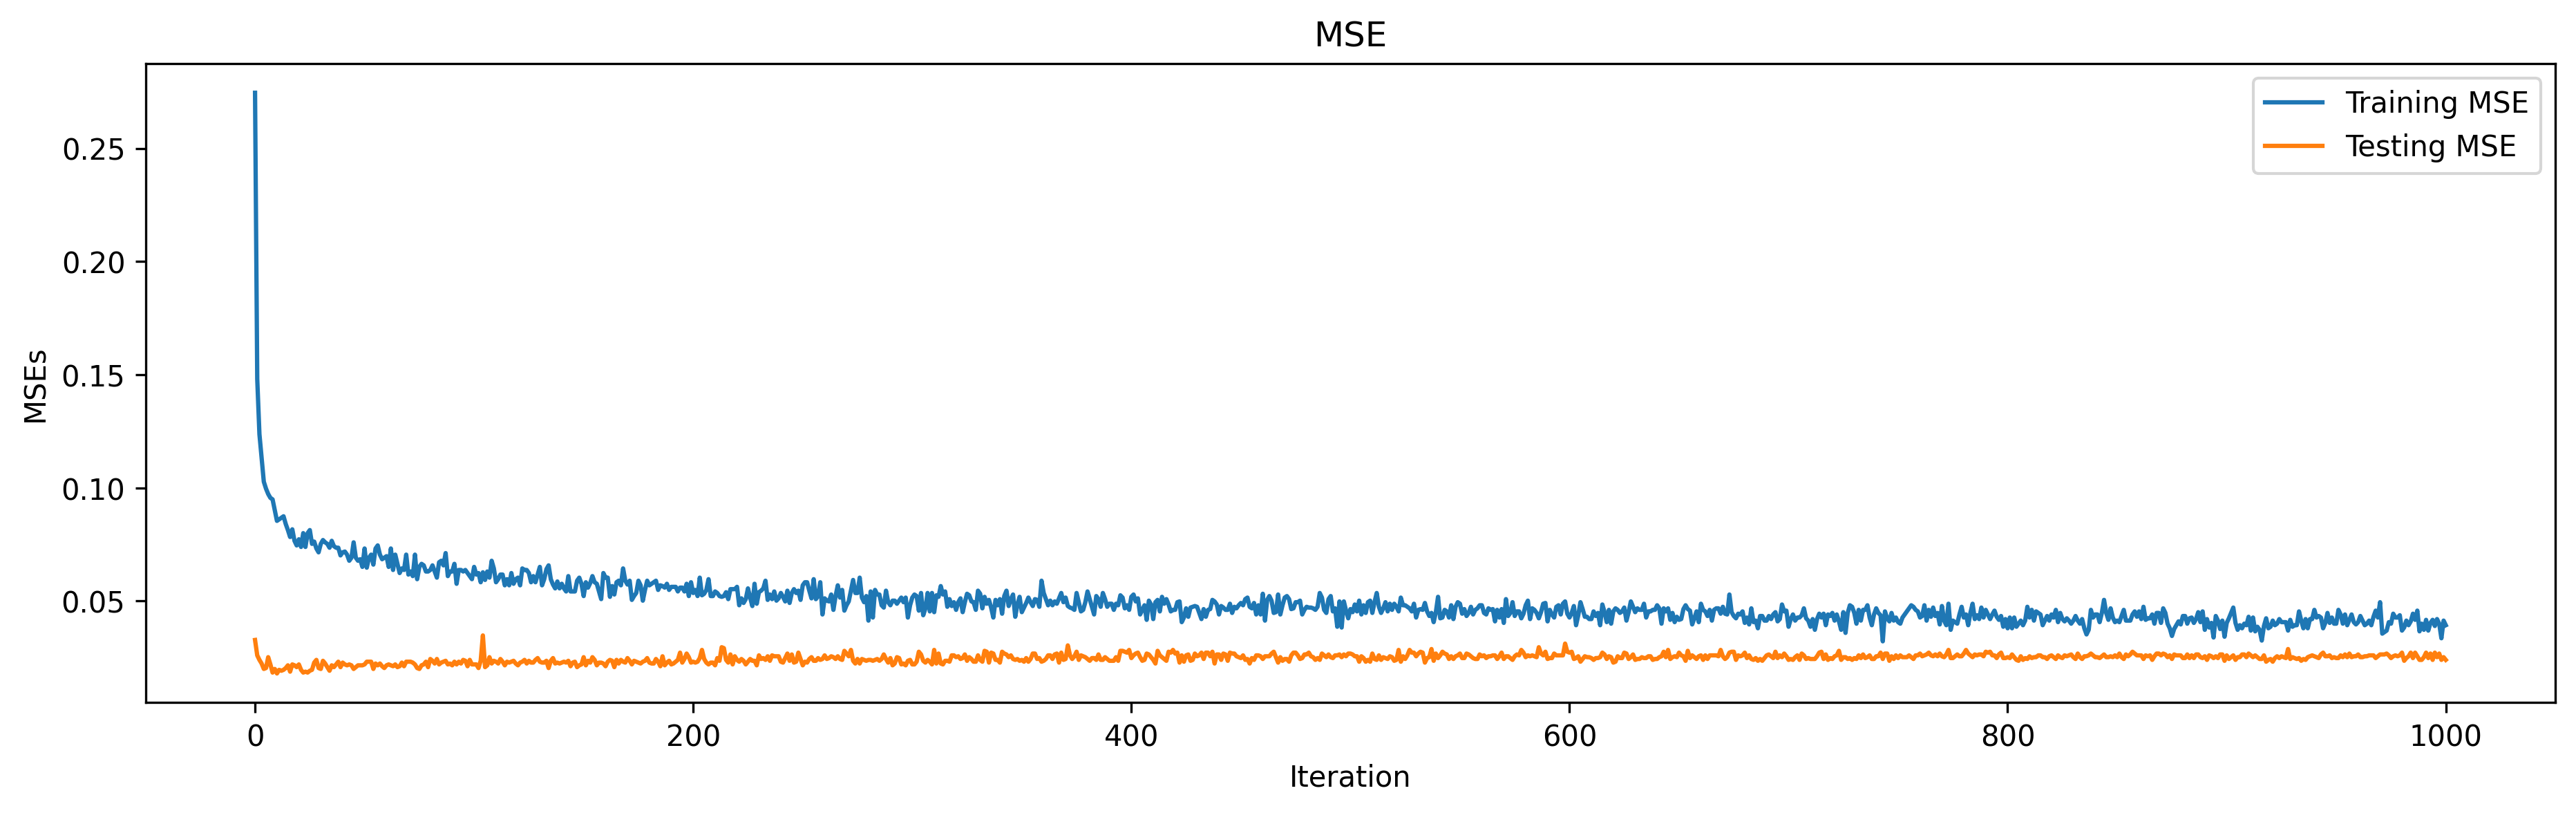
\includegraphics[width=\textwidth]{./plots/plot5.png}
    \caption{Training vs Testing Mean Square Error (MSE).}
    \label{fig:plot4}
\end{figure}

On one hand it is clear that peak accuracy is achieved at 10-20 iterations, after which the reduction in training MSE seems to indicate overfitting rather than actual improvement.
Since the weights are randomly initialized at each run, multiple runs equal to simulated annealing and can serve to expose entrapment to local minimum.
As the MSE is repeatedly similar, we can infer that the algorithm does not converge to a poor local minimum.

Given the baseline MSE calculated in the notepad as 3.6, it is evident that the model has actually learned to distinguish between the two classes (8 and 9).
The weights matrix has the same properties as the input matrix and thus, be reversing the process of transforming the digit images to input arrays, we can produce an image of the learned weights.
Figure 5a provides this visualization, and makes clear that this particular simple model does not learn any high level features a human would use.
Instead it may opportunistically utilize whichever pixels help it correctly split groups of samples that the training so far has not been able to assist it with, similar to nodes that split high impurity leaves in decision trees.
Figure 4 shows the difference between the average image of 8 and 9.
Areas with high or low brightness indicate consistent differences between the classes that could be used for a rule based system, yet we see that the model has focused elsewhere.

\begin{figure}[h!]
    \centering
    \begin{subfigure}[t]{0.3\textwidth}
        \centering
        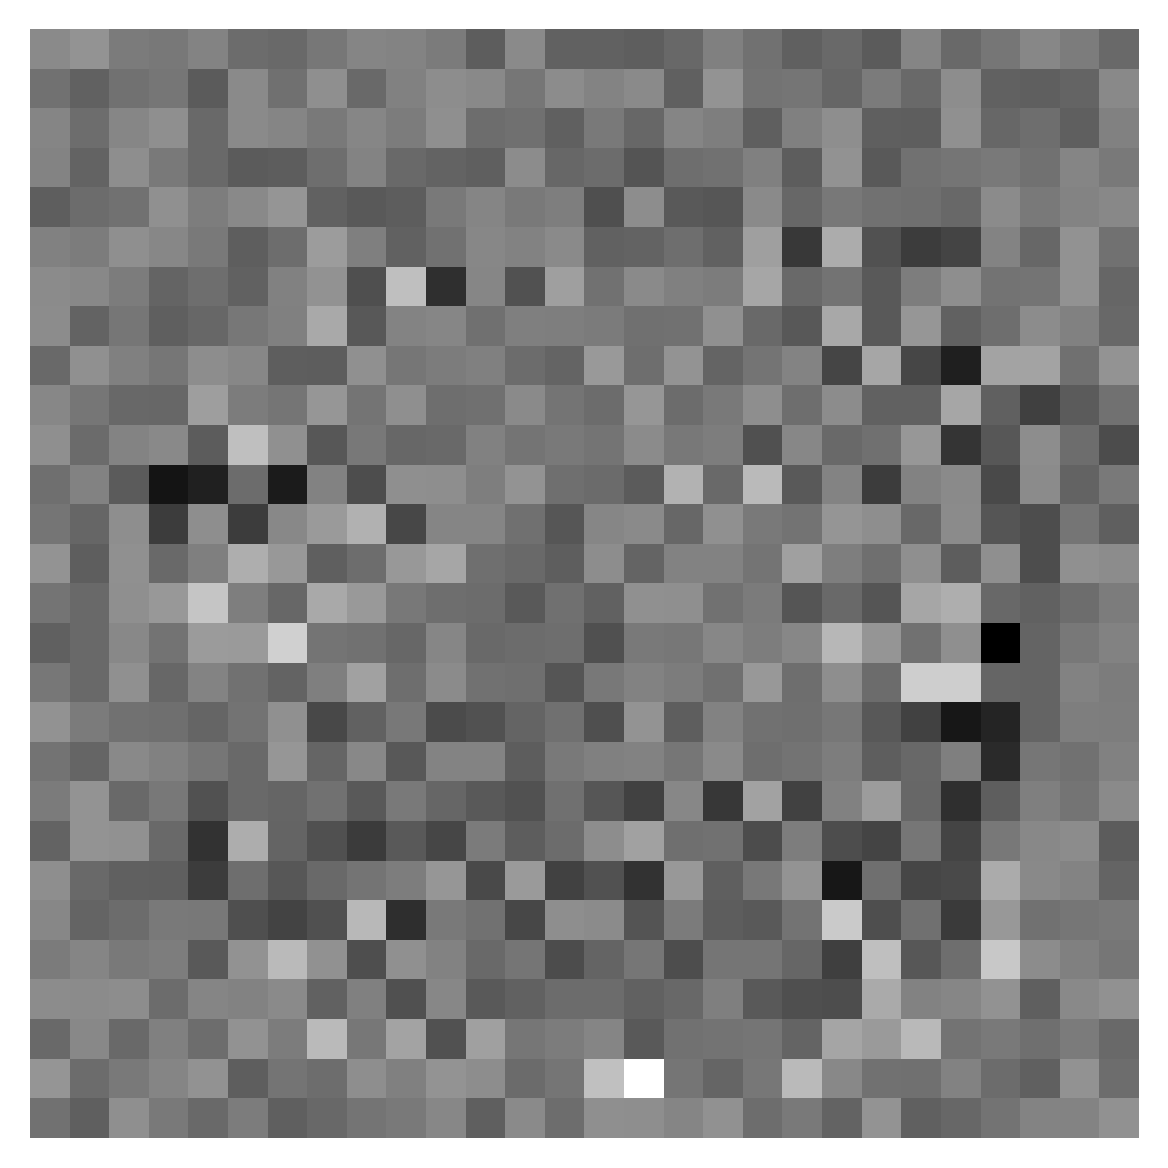
\includegraphics[width=\textwidth]{./plots/plot6.png}
        \caption{Visualisation of weights learned by the Perceptron}
        \label{fig:plot5a}
    \end{subfigure}
    \hspace{0.01\textwidth}
    \begin{subfigure}[t]{0.3\textwidth}
        \centering
        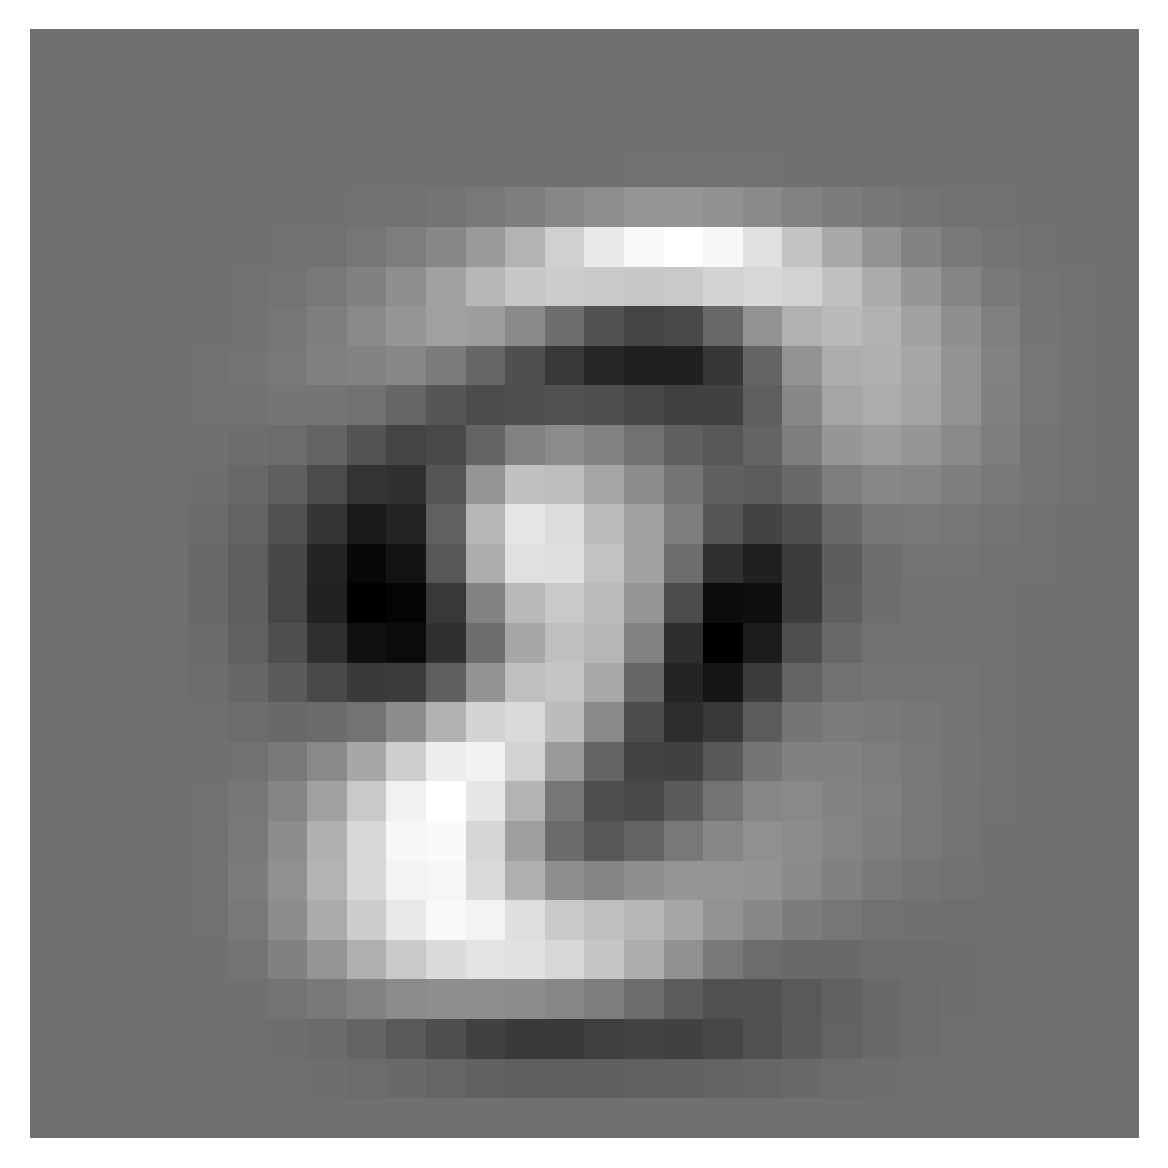
\includegraphics[width=\textwidth]{./plots/plot7.png}
        \caption{Difference between average hand-drawn 8 and 9 characters}
        \label{fig:plot5b}
    \end{subfigure}
    \hspace{0.01\textwidth}
    \begin{subfigure}[t]{0.3\textwidth}
        \centering
        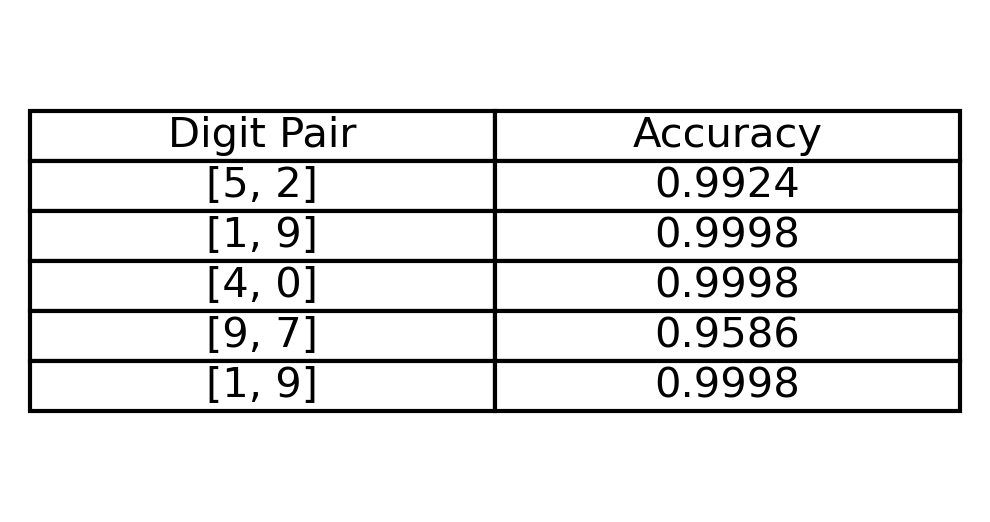
\includegraphics[width=\textwidth]{./plots/plot8.png}
        \caption{Accuracies for various digit pairs}
        \label{fig:plot5c}
    \end{subfigure}
    \caption{How the model 'sees' the samples vs How we would expect it to see. Achieved accuracies for random pairs}
    \label{fig:plot5}
\end{figure}

Figure 6 is a compilation of other pairs of digits with the respective achieved accuracy after training.
We see variations that are aligned with how visually similar the two digits are, (that is the handwritten versions as the digital ones can differ e.g. handwritten '5' often lookls more like an 'S'

\section{Multilayer Perceptrons (Task 3)}

To solve the problem of the perceptron’s simplicity, we can organize large groups of them into Neural Networks (NN).
The motivation stems from a property called “emergence” where the capabilities of a structure exceed the sum of its parts (Pedder, 2023).
In the software domain, the model can learn complex curves to separate the classes more effectively than hyperplanes can (Choi, 2020).
While setting up the network with the Keras Library, there are multiple hyperparamters to select. 
Number of epochs is similar to the iterations in task 2, and batch size allows the model to work with groups of samples speeding up training.
The amount of time needed to find the best combination increases exponentially so using guidelines (Bengio, 2012) and some tests, we find one that is sufficient.
The resulting training and test accuracy is as follows:.

\begin{figure}[h!]
    \centering
    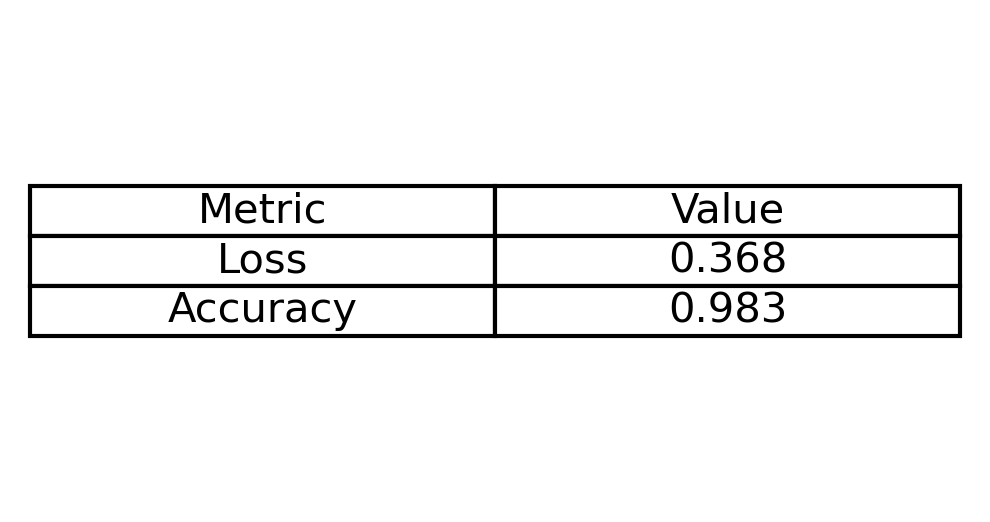
\includegraphics[width=0.3\textwidth]{./plots/plot10.png}
    \caption{MLP accuracy on train and test datasets}
    \label{fig:plot6}
\end{figure}

At first sight it might seem as if the accuracy is lower that with the perceptron.
However, the model now performs multiclass classification, not binary classification, which is significantly more demanding.

\begin{figure}[h!]
    \centering
    \begin{subfigure}[t]{\textwidth}
        \centering
        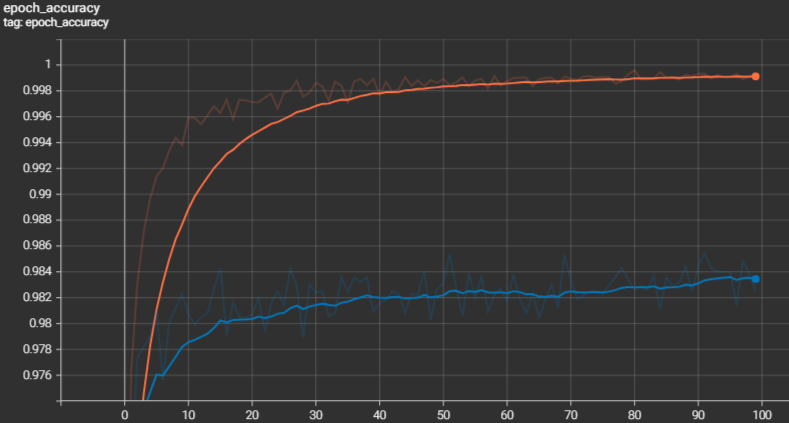
\includegraphics[width=0.7\textwidth]{./plots/screenshot1.png}
        \caption{Train (yellow) and test (blue) accuracy at each epoch.}
        \label{fig:fig7a}
    \end{subfigure}
    \vspace{0.2cm}
    \begin{subfigure}[t]{\textwidth}
        \centering
        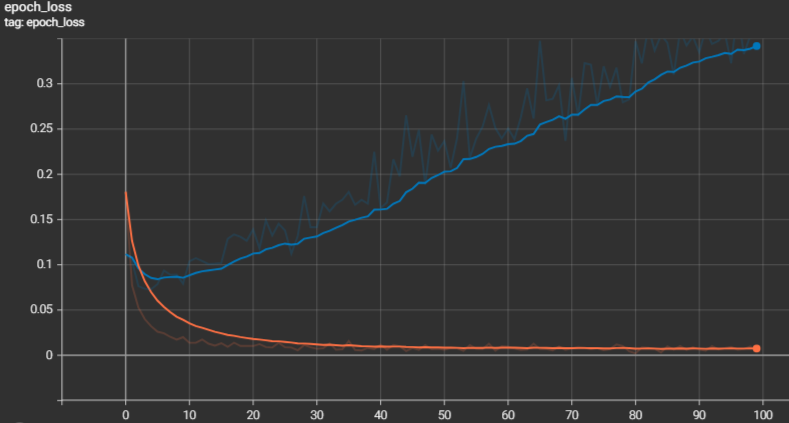
\includegraphics[width=0.7\textwidth]{./plots/screenshot2.png}
        \caption{Train (yellow) and test (blue) loss at each epoch.}
        \label{fig:fig7b}
    \end{subfigure}
    \caption{Train and test metrics vs epochs for standard MLP. Smoothing is set to 0.9.}
    \label{fig:plot7}
\end{figure}

We leave the model to train for 100 epochs to monitor accuracy and loss.
We can see that accuracy score on the validation dataset gets close to its maximum within 30 epochs, but does not stop improving till the end, albeit very slowly.
On the other hand, test loss reaches it minimum at around 5 epochs, after which it steadily increases while training loss keeps reducing, indicating overfitting.
It is noteworthy that comparing (validation) accuracy and loss we get contradicting results.
This is due to the fact that loss evaluates the output probabilities while accuracy evaluates the results.
As the model overfits, the model becomes “confused” and less certain but not so much so that it completely misses the target (Smith, 2017).

Next we investigate the relationship between network layers and accuracy by training and testing multiple MPLs of various depths with all other hyperparameters constant
The number of neurons per layer is decreased to 500 to achieve training in reasonable time.
We produce 4 models with 3, 4, 6 and 8 such layers.

\begin{figure}[h!]
    \centering
    \begin{subfigure}[t]{\textwidth}
        \centering
        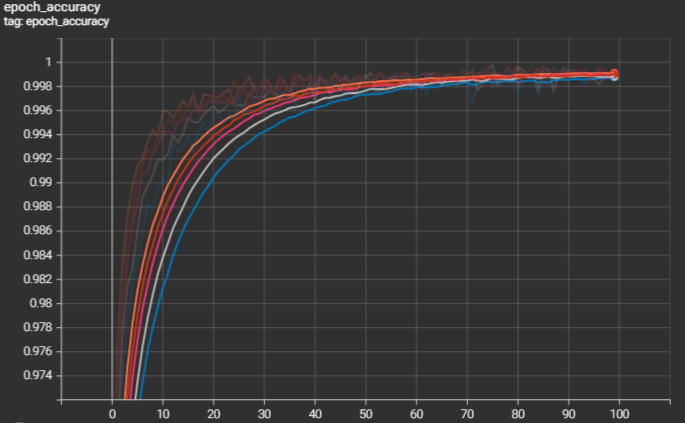
\includegraphics[width=0.7\textwidth]{./plots/screenshot3.png}
        \caption{Train accuracies for all models.}
        \label{fig:subfig8a}
    \end{subfigure}
    \vspace{0.2cm}
    \begin{subfigure}[t]{\textwidth}
        \centering
        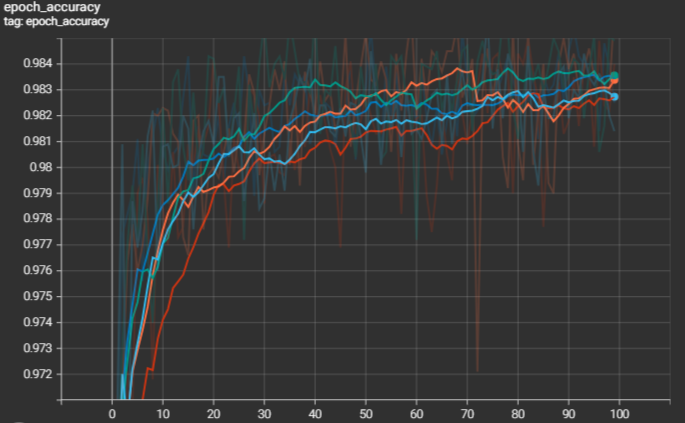
\includegraphics[width=0.7\textwidth]{./plots/screenshot4.png}
        \caption{Test accuracies for all models.}
        \label{fig:subfig8b}
    \end{subfigure}
    \vspace{0.2cm}
    \begin{subfigure}[t]{\textwidth}
        \centering
        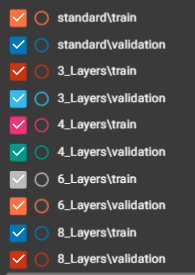
\includegraphics[width=0.12\textwidth]{./plots/screenshot5.png}
        \label{fig:subfig8c}
    \end{subfigure}
    \caption{Train and test accuracies of all models. Smoothing is set to 0.9.}
    \label{fig:plot8}
\end{figure}

Looking at the train curves, we see that the train performance decreases with each added layer, indicating overfitting.
The fact that the standard model is still the best could indicate that trading "width for "depth" is the wrong thing to do here.
Similar things apply for the test dataset but with less consistency.
The differences are of the order of \(0.1\% \) and there is some randomness involved (wheights init, train/test split), but the trend is reproducable accross different runs, so it would appear that all models hit a ceiling at around \(98.3\%\) accuracy (vanishing gradient stops training after a depth).
We would expect some drop to accuracy for deeper models owning to overfiting but as we saw before, the degradation to performance appears on the loss.

Regarding the number of parameters for each model, the results are as follows:
For fully connected layers, each neuron corresponds to one parameter for each input, plus the bias. Therefore, for the first layer, we calculate:
\[
(784+1) \cdot 500 = 392,500.
\]
Subsequently, each layer adds:
\[
(500+1) \cdot 500 = 250,500
\]
parameters, and the softmax layer adds:
\[
(500+1) \cdot 10 = 5,010
\]
parameters. 

Thus, the total number of parameters works out to:
\[
397,510 + 250,500 \cdot n,
\]
where \(n\) is the number of layers.

We can plot these values along with the respective accuracies.

\begin{figure}[h!]
    \centering
    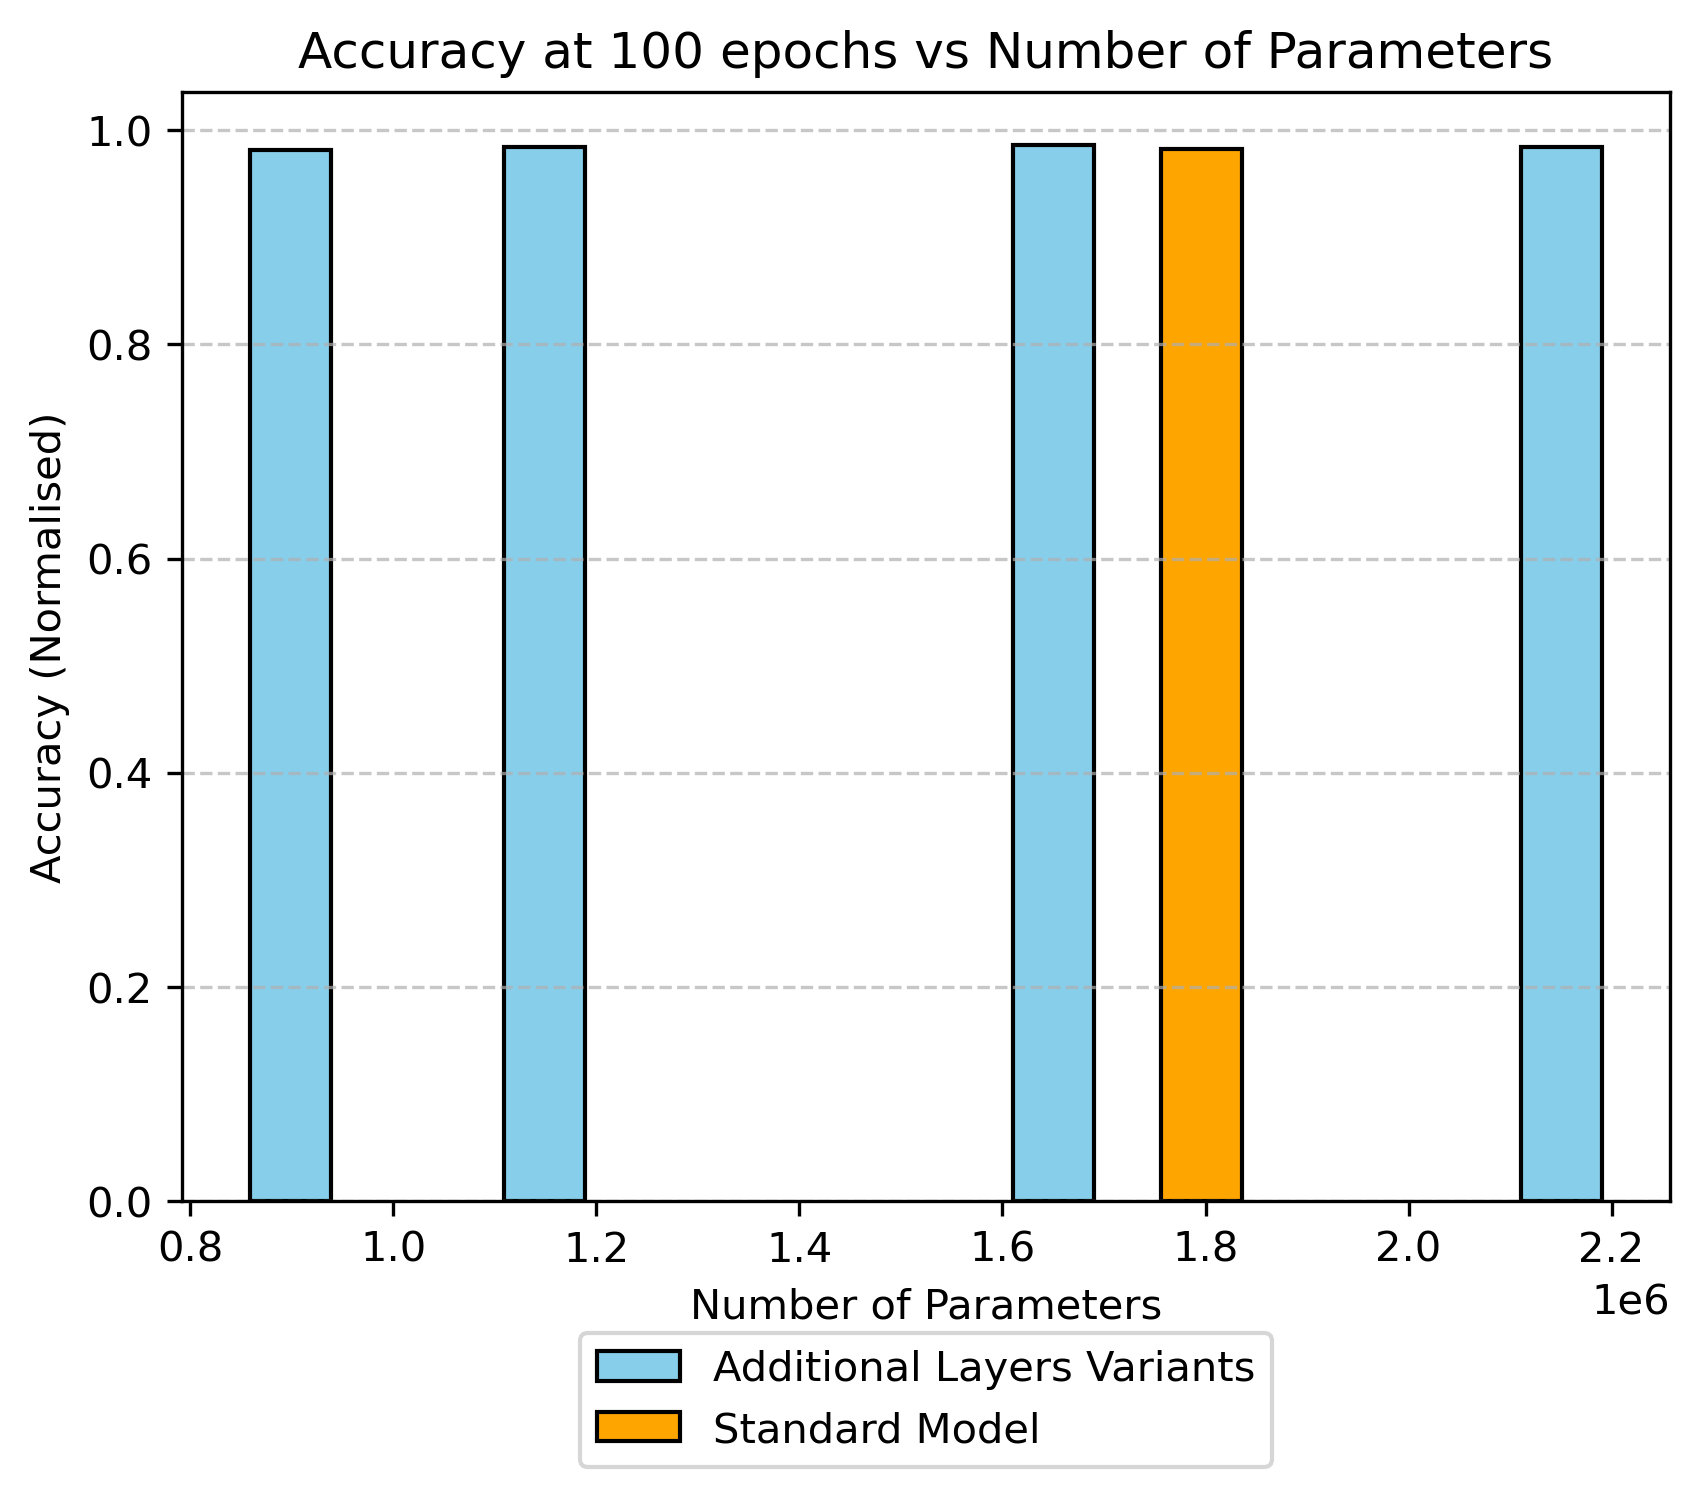
\includegraphics[width=0.8\textwidth]{./plots/plot11.png}
    \caption{Accuracy for different architectures. No linear trend apparent but the models in the center seem to perform slightly better.}
    \label{fig:plot9}
\end{figure}

The main model is second with most parameters because of the wider layers.
At the large scale of things, all architectures perform similarily in terms of accuracy and as discussed, overfitting manifests itself as higher loss only.
We conclude that for this problem, lighter configurations would be beneficial.

\section{Convolutional Neural Networks (Task 4)}

Convolutional Neural Networks (CNNs) perform calculations on groups of features instead of individual ones.
The calculation uses a kernel, that is a matrix of weights, that gets applied on the similarily sized slices of the sample using the rolling window approach.
More specifically, each value of the kernel is mulitplied with the respective value of the sample's matrix. with all the products being summed.
That means that the applied calculations now take geometry or time (or other forms of oganisation) into account.
The produced output is a map of the places where the structure of the kernel is found in the original image.

\begin{figure}[h!]
    \centering
    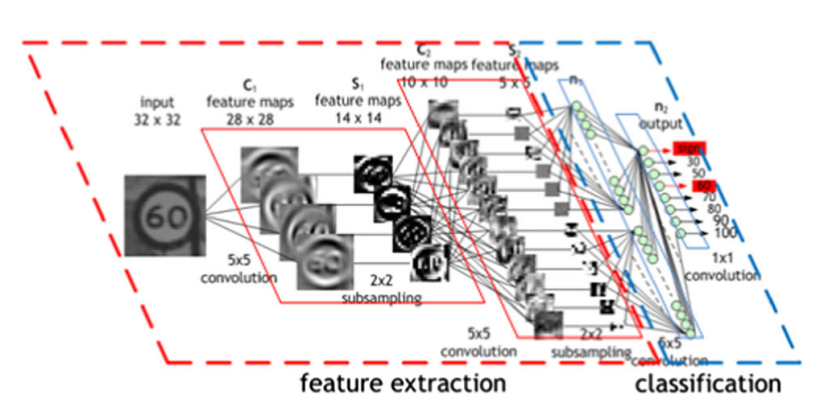
\includegraphics[width=0.8\textwidth]{./plots/screenshot6.png}
    \caption{Application of the left sobel matrix highlights vertical high to low transitions of the face image (Powell)}
    \label{fig:plot10}
\end{figure}

In a typical CNN architecture, multiple kernels are applied to the input layer which itself may consist of multiple layers.
The kernels match the input in terms of depth as well and each kernel produces an additional layer for the output. These are visualised in figure 11

\begin{figure}[h!]
    \centering
    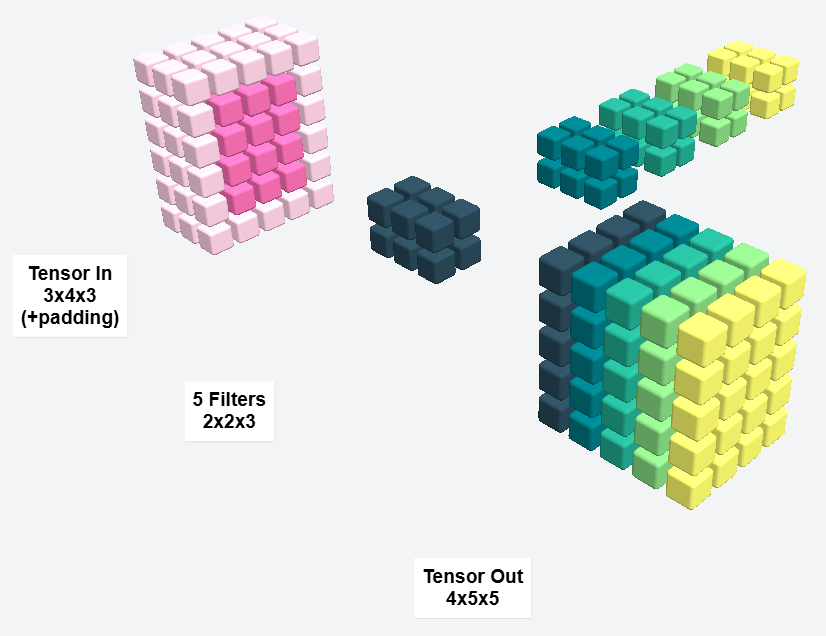
\includegraphics[width=0.8\textwidth]{./plots/screenshot7.png}
    \caption{Characteristics of input and output layers in CNNs (made with Convviz)}
    \label{fig:plot11}
\end{figure}

This array of extracted features can then be used by higher order layers to synthesize more complex features, allowing the identification of complex entities.
An example is shown in figure 12 where speed signs are identified as specific combinations of simpler shapes.

\begin{figure}[h!]
    \centering
    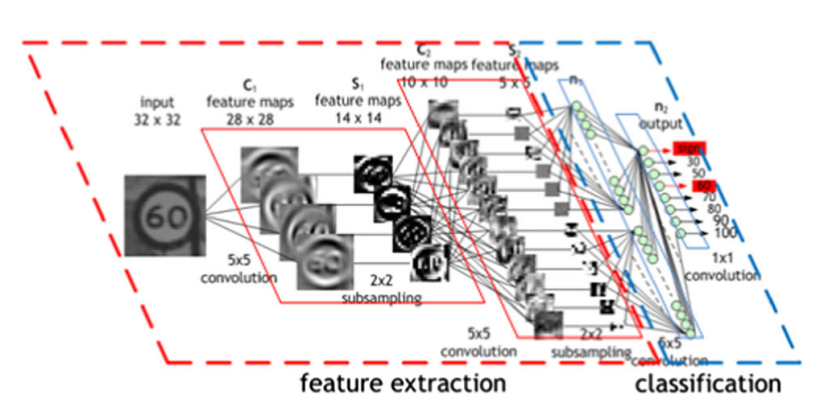
\includegraphics[width=0.8\textwidth]{./plots/screenshot8.png}
    \caption{The CNN uses simple features (like the left sobel from figure 10) to construct complex ones (Ghoshal, 2020)}
    \label{fig:plot12}
\end{figure}

\begin{figure}[h!]
    \centering
    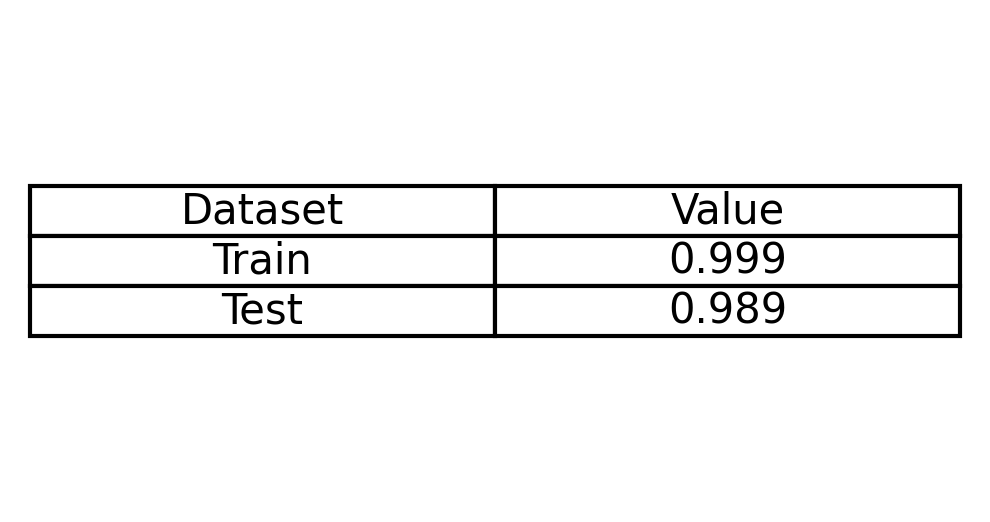
\includegraphics[width=0.3\textwidth]{./plots/plot12.png}
    \caption{CNN accuracy on train and test datasets}
    \label{fig:plot13}
\end{figure}

We see that the CNN model performs better on the test dataset than any of the MLPs.
Plotting the train and test accuracies with tensorboard in figure 14, we can see that for the test data, peak accuracy is reached after 6 epochs.
After that, training accuracy keeps increasing while test accuracy has a slight downwards trend, indicating overfiting.

\begin{figure}[h!]
    \centering
    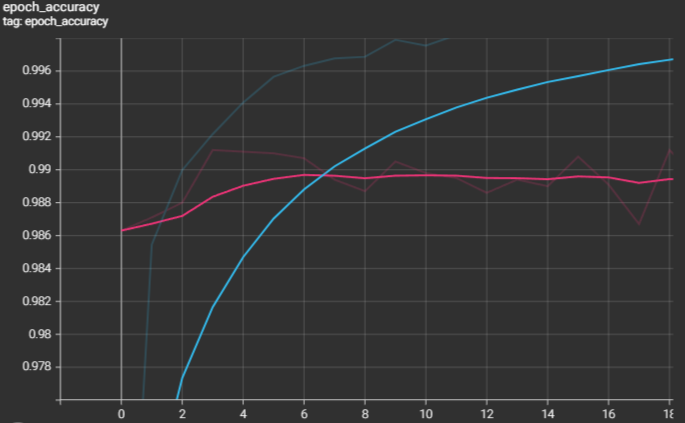
\includegraphics[width=0.7\textwidth]{./plots/screenshot9.png}
    \caption{Train (cyan) and test (pink) accuracy at each epoch.}
    \label{fig:plot14}
\end{figure}

We will now make alterations to the Standard model to see how different hyperparameters affect it's behaviour.
Focusing less on the initial epochs, the first thing that stands out is that increasing the kerne size from (4, 4) to (5, 5) is the only tweak that actually harms the accuracy
Increasing the model's depth by adding a fourth layer (without other layers like pooling, normalisation, attention etc) seems to be the best tweak, though the increased number of parameters makes training slower. 
Same goes for the wider version.
In addition, these two variants maintain the upwards trend till the end, sugesting that more iterations could further benefit them. However this is also true for the worse (bigger kernel) one.
The narrower model seems to perform as well as the standard one.
In general the difference between the best and worse models is \(0.2\%\) and some noise exists in these results as the experiment was only repeated once.
Hence the safer conclusions are deeper and wider are better than bigger kernel for similar number of epochs.
However, given more time, more models would be allowd the reach their full potential so the results could be different then.
Also, the number of trainable parameters is vastly different between architectures so a performance/parameter graph must also be considered.

\begin{figure}[h!]
    \centering
    \begin{subfigure}[t]{\textwidth}
        \centering
        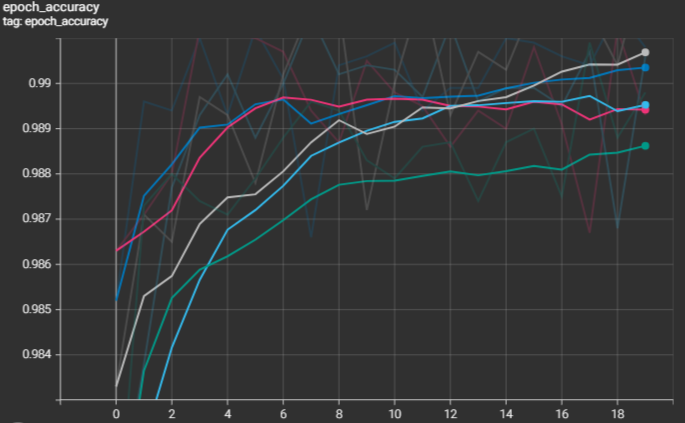
\includegraphics[width=0.7\textwidth]{./plots/screenshot10.png}
        \caption{Test accuracies for all CNN models.}
        \label{fig:subfig15a}
    \end{subfigure}
    \vspace{0.2cm}
    \begin{subfigure}[t]{\textwidth}
        \centering
        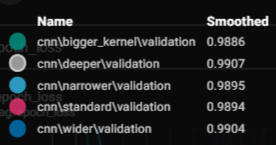
\includegraphics[width=0.3\textwidth]{./plots/screenshot11.png}
        \caption{Legand.}
        \label{fig:subfig15b}
    \end{subfigure}
    \caption{Test accuracies of all CNN models. Smoothing is set to 0.9.}
    \label{fig:plot15}
\end{figure}

To calculate the number of parameters in a CNN, we have that each \(n \cdot n \cdot k\) kernel has
\[
n \cdot n \cdot k + 1 = n^2 \cdot k + 1.
\]
parameters, where k is the depth of the layer and we take into account the bias. 

Hence, for the 32 filters of the first layer we have
\[
(4 \cdot 4 \cdot 1) \cdot 32 + 32 = 544.
\]
parameters. For the following layers, we need to adjust for the different depths which are now 32 instead of 1 for input and 64 instead of 32 for output:
\[
(4 \cdot 4 \cdot 32) \cdot 64 + 64 = 32,832.
\]

With similar logic we get
\[
131,200
\]
for the last convolutional layer.

The flatten layer has no parameters. So far we have ignored the stride and padding (which is zero) as they only affect the dense layer.
In the general case, the size of the input after a convolutional layer becomes:
\[
\text{Output size} = \frac{\text{Input size} - \text{Kernel size} + 2 \cdot \text{Padding}}{\text{Stride}} + 1
\]
so for the stride of 1 of the first layer we get
\[
\text{First layer output} = \frac{28 - 4 + 2 \cdot 0}{1} + 1 = 25.
\]
This becomes 
\[
\text{Second layer output} = \frac{25 - 4 + 2 \cdot 0}{2} + 1 = 11.
\]
as divisions are rouded down. Finally we get:
\[
\text{Third layer output} = \frac{11 - 4 + 2 \cdot 0}{2} + 1 = 4.
\]
hence the flat layer produces 
\[
(4 \cdot 4 \cdot 128) = 2,048 \text{ values}.
\]
Now, the dense layer calculates 10 parameters for each, plus 10 biases for each neuron, which results in
\[
2,048 \cdot 10 + 10 = 20,490 \text{ parameters}.
\]


With similar logic we can calculate the number of parameters of all variations, or simply extract them with the provided method.
Ploting the Accuracy over Number of Parameters we get Figure 16. On (a) we see that, as expected, the higher performing models posses more parameters.
(b) shows that better accuracy is achieved with more trainig time, but the relation is not linear and the tradeoff is questionable when 0.1\% improvement requires more that twice the training time.
From (c) we see that surprisingly, trainig time is not linear with number of parameters. This is because the wider one has more filters, all of which are processed for each value of each filter.

\begin{figure}[h!]
    \centering
    \begin{subfigure}[t]{0.3\textwidth}
        \centering
        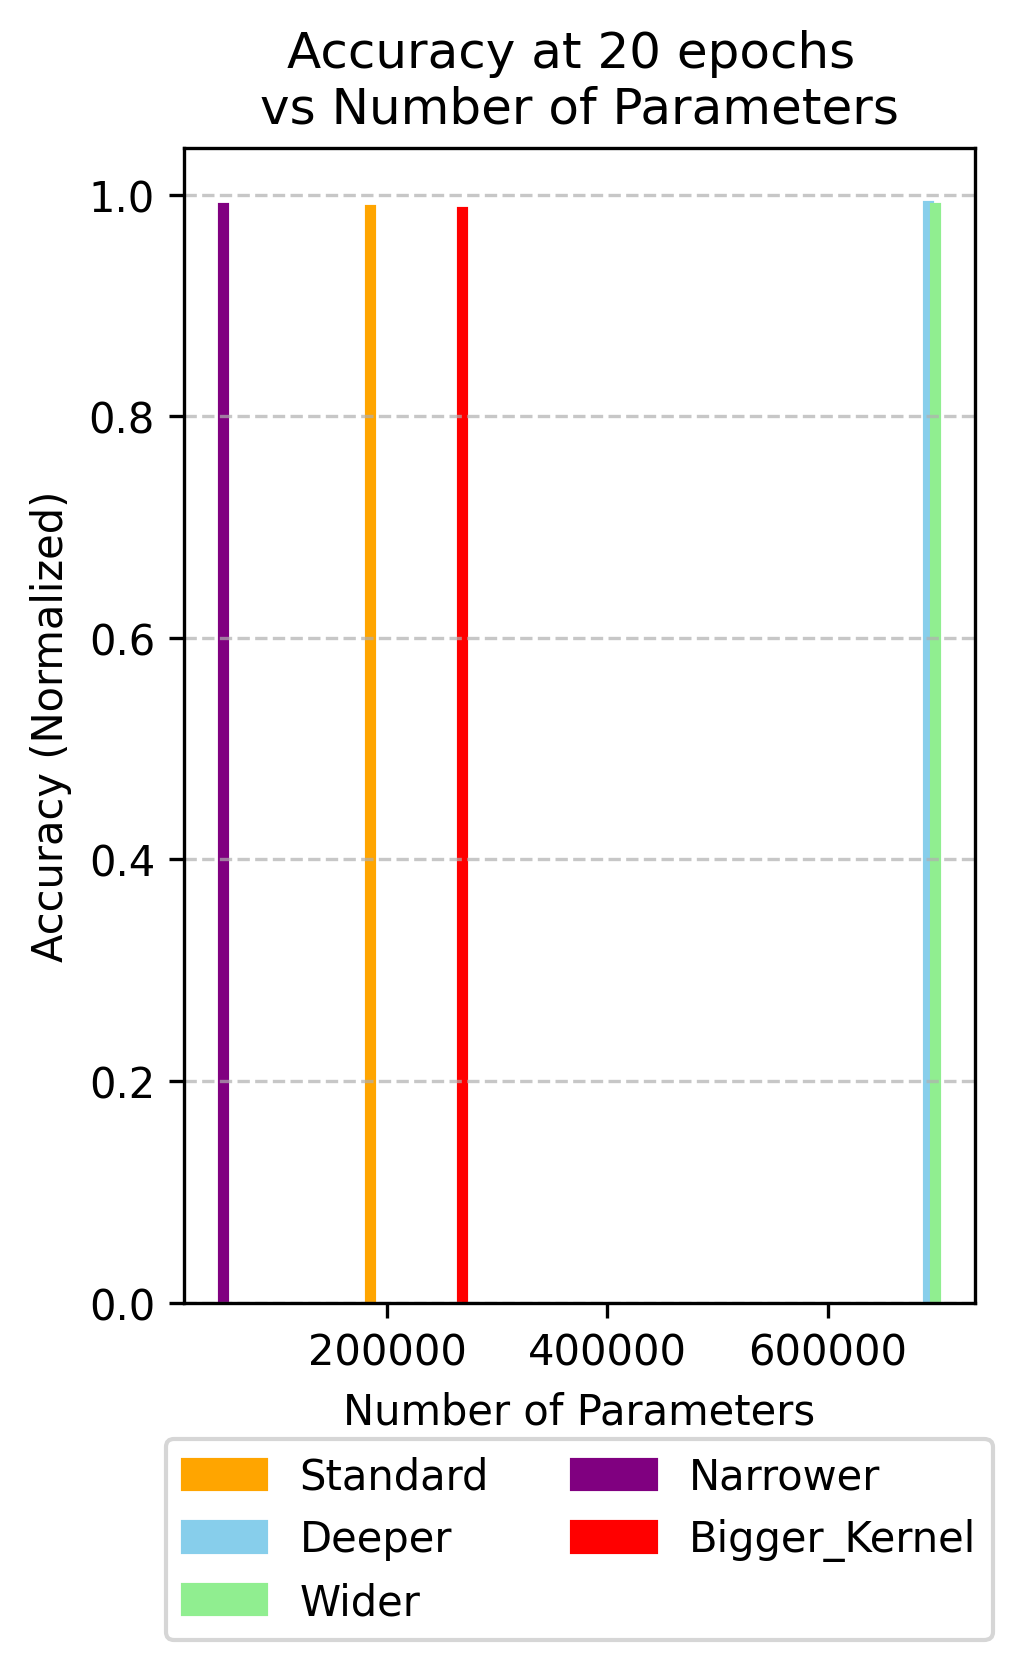
\includegraphics[width=\textwidth]{./plots/plot13.png}
        \caption{Accuracy vs Parameters}
        \label{fig:plot16a}
    \end{subfigure}
    \hspace{0.01\textwidth}
    \begin{subfigure}[t]{0.3\textwidth}
        \centering
        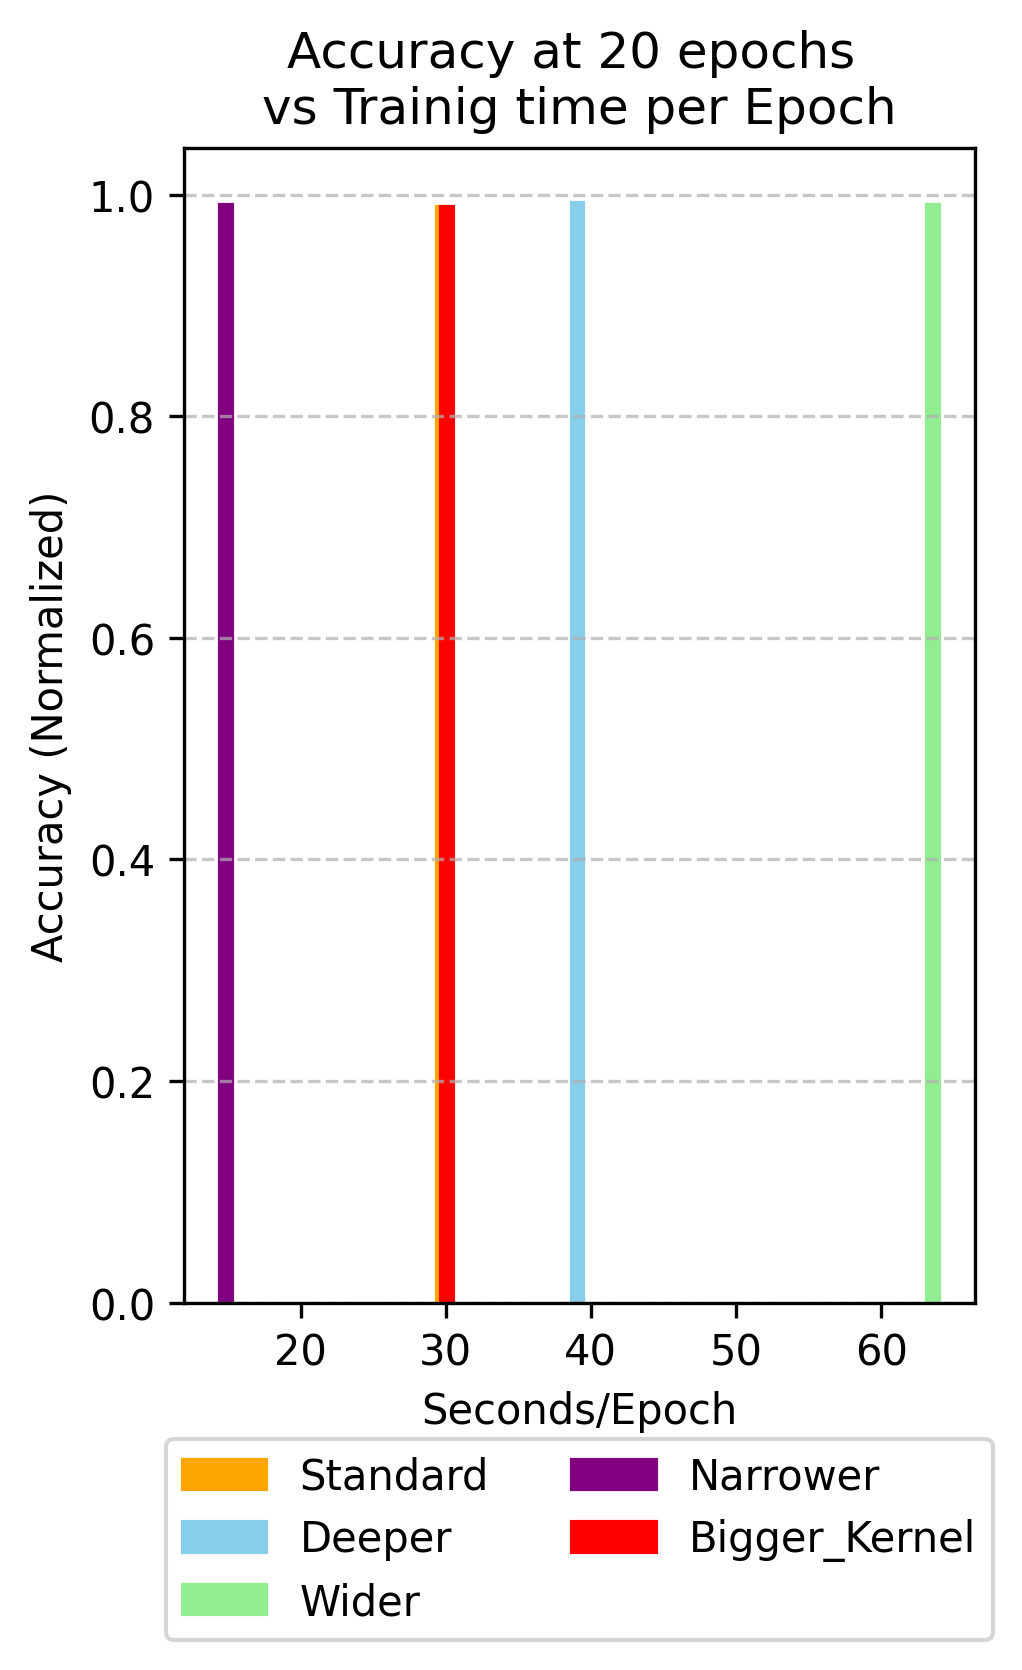
\includegraphics[width=\textwidth]{./plots/plot14.png}
        \caption{Accuracy vs Training Time}
        \label{fig:plot16b}
    \end{subfigure}
    \hspace{0.01\textwidth}
    \begin{subfigure}[t]{0.3\textwidth}
        \centering
        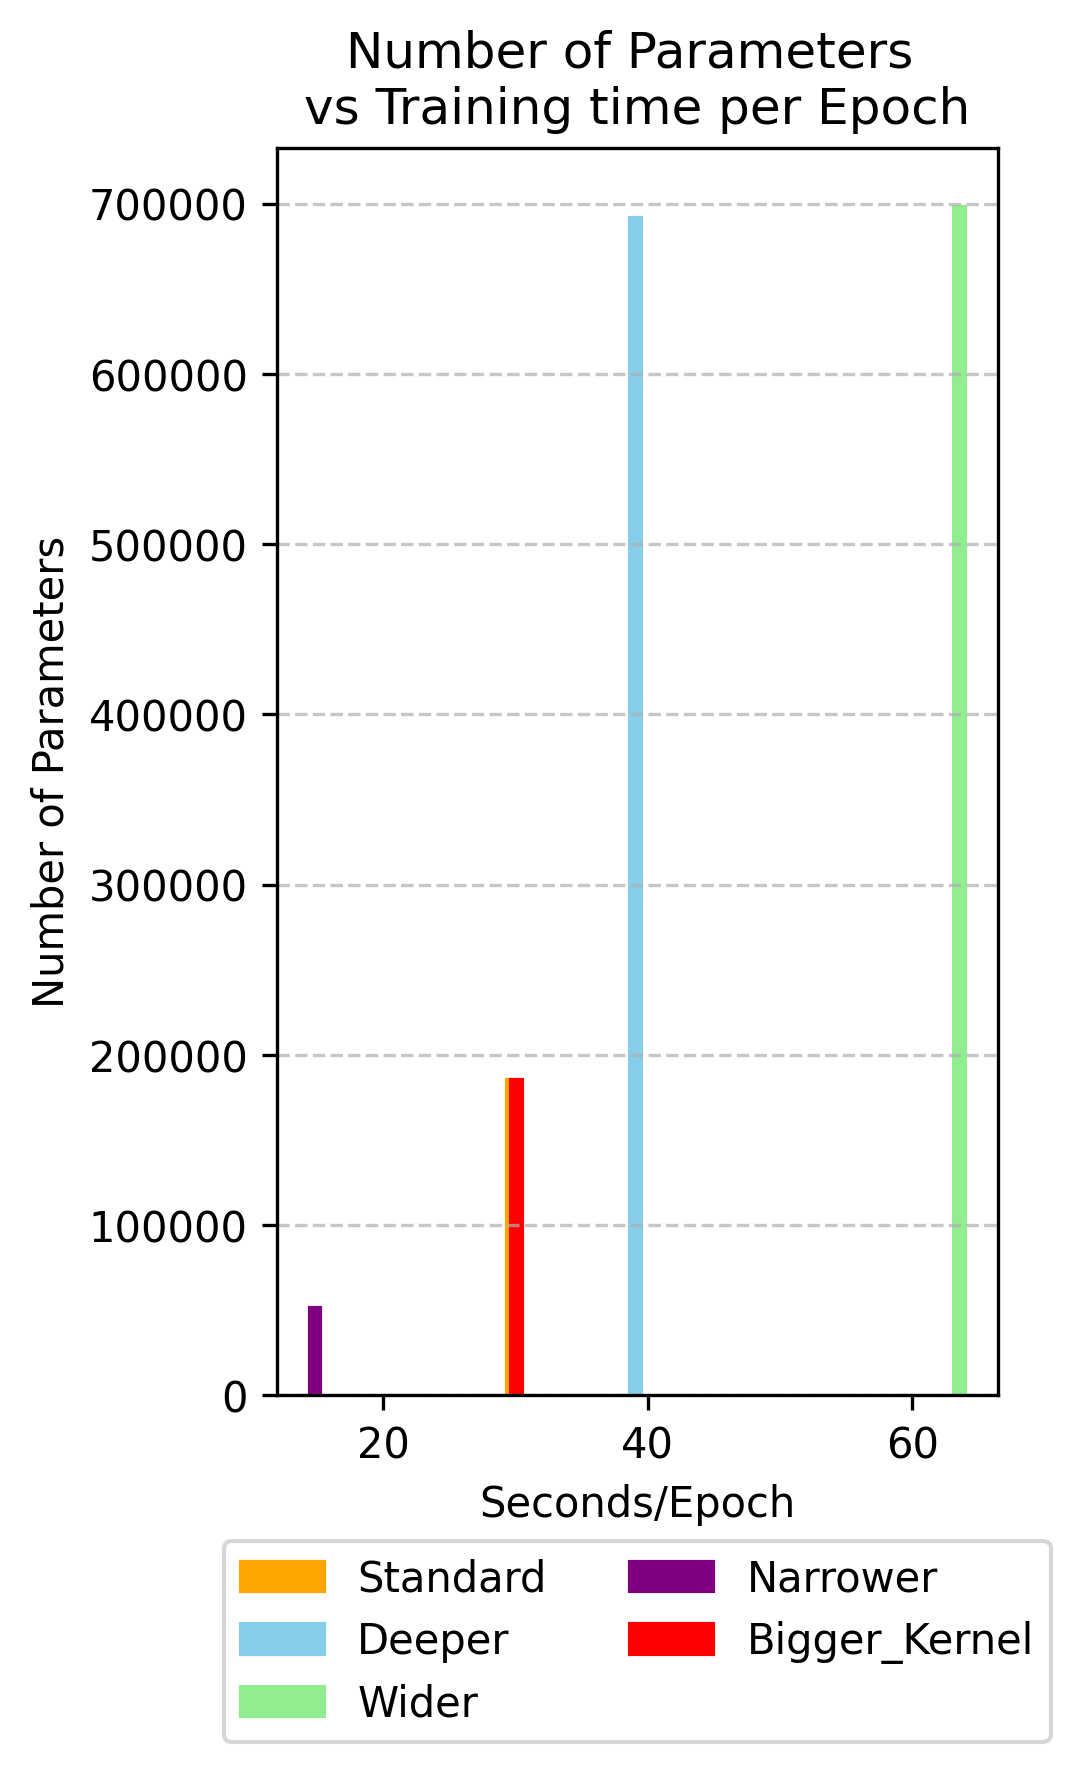
\includegraphics[width=\textwidth]{./plots/plot15.png}
        \caption{Parameters vs Training Time}
        \label{fig:plot16c}
    \end{subfigure}
    \caption{Comparison of Accuracy, Number of Parameters and Training Time}
    \label{fig:plot16}
\end{figure}

Compared to MLPs, we see that the performance is better with way less parameters but more training time, as convolutions and back propagation accross many filters and windows are more compute intensive that matrix multiplications


\section{Visualising CNN outcomes (Task 5)}

Our standard CNN architecture has 3 convolutional layers. Each layer needs as many kernels as the number of input layers, and that is repeated for each output filter of that layer.
Hence, the first layer has 32 filters, the second layer has 64 filters for each of the 32 filters of the previous layer, and the third one has \(128 \cdot 64\) filters.
All filters are \(4\times4\) since thats the difined kernel size

\begin{figure}[h!]
    \centering
    \begin{subfigure}[t]{0.3\textwidth}
        \centering
        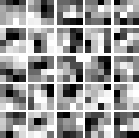
\includegraphics[width=\textwidth]{./plots/layer_0_plot.png}
        \caption{Filters from convolution layer 0.}
        \label{fig:subfig17a}
    \end{subfigure}
    \hfill
    \begin{subfigure}[t]{0.3\textwidth}
        \centering
        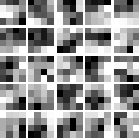
\includegraphics[width=\textwidth]{./plots/layer_1_plot.png}
        \caption{Filters from convolution layer 1.}
        \label{fig:subfig17b}
    \end{subfigure}
    \hfill
    \begin{subfigure}[t]{0.3\textwidth}
        \centering
        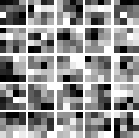
\includegraphics[width=\textwidth]{./plots/layer_2_plot.png}
        \caption{Filters from convolution layer 2.}
        \label{fig:subfig17c}
    \end{subfigure}
    \caption{Filters from all layers, arranged side by side.}
    \label{fig:plot17}
\end{figure}



We show 25 filters from each layer so that includes both lower and higher level features.
Because of the small kernel size, it is difficult to identify specific part of some digit.
What we notice instead are motifs of stark differences. 
In layer 0 these are used to identify smaller details are different between digits.
In higher layers the filters identify the distribution of the previous levels finer details.

\begin{figure}[h!]
    \centering
    \begin{subfigure}[t]{0.3\textwidth}
        \centering
        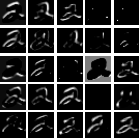
\includegraphics[width=\textwidth]{./plots/activation2_0.png}
        \caption{Activations from convolution layer 0.}
        \label{fig:subfig18a}
    \end{subfigure}
    \hfill
    \begin{subfigure}[t]{0.3\textwidth}
        \centering
        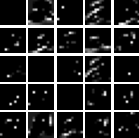
\includegraphics[width=\textwidth]{./plots/activation2_1.png}
        \caption{Activations from convolution layer 1.}
        \label{fig:subfig18b}
    \end{subfigure}
    \hfill
    \begin{subfigure}[t]{0.3\textwidth}
        \centering
        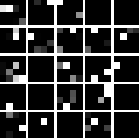
\includegraphics[width=\textwidth]{./plots/activation2_2.png}
        \caption{Activations from convolution layer 2.}
        \label{fig:subfig18c}
    \end{subfigure}
    \caption{Activations for random sample '2'}
    \label{fig:plot18}
\end{figure}

\begin{figure}[h!]
    \centering
    \begin{subfigure}[t]{0.3\textwidth}
        \centering
        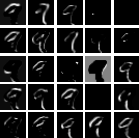
\includegraphics[width=\textwidth]{./plots/activation9_0.png}
        \caption{Activations from convolution layer 0.}
        \label{fig:subfig19a}
    \end{subfigure}
    \hfill
    \begin{subfigure}[t]{0.3\textwidth}
        \centering
        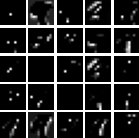
\includegraphics[width=\textwidth]{./plots/activation9_1.png}
        \caption{Activations from convolution layer 1.}
        \label{fig:subfig19b}
    \end{subfigure}
    \hfill
    \begin{subfigure}[t]{0.3\textwidth}
        \centering
        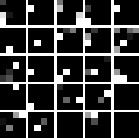
\includegraphics[width=\textwidth]{./plots/activation9_2.png}
        \caption{Activations from convolution layer 2.}
        \label{fig:subfig19c}
    \end{subfigure}
    \caption{Activations for random sample '9'}
    \label{fig:plot19}
\end{figure}

Figures 18 and 19 show the the activations of 8 kernels for each convolutional layer.
We see that the activations of the first layer create a sort of partial outline of the digit, a map of where a specific patern is present.
Hence, while they still resemble the drawing, new shapes are created.
The following layers do not "look" at the image but instead at the activation maps (the new shapes) and thus are not recogniseable, but they start to look more like the filters from Figure 17.
We could say that the model manages to circumvent some of the noise that comes with human hand drawing by creating and using custom features that are invariable.

\section{Acknowledgments}
For some complex Matplotlib plots, OpenAI's ChatGPT model 4o was used to assist with the code's syntax.


\section{References}

Khee, L. K., 2022. \textit{Limitation of Data Visualisation} [Online]. Available from 
\href{https://medium.com/@e0673935/limitation-of-data-visualization-1e4db068a22a}{https://medium.com/@e0673935/\newline limitation-of-data-visualization-1e4db068a22a} [Accessed 13 October 2024]. \newline

\noindent
Mackiewicz, A., Ratajczak, W., 1993. Principal Components Analysis. \textit{Computers \& Geosciences}, 19(3), 303-342. \newline

\noindent
Shahapure, K. R., Nicholas, C., 2020. Cluster Quality Analysis Using Silhouette Score. \textit{2020 IEEE 7th International Conference on Data Science and Advanced Analytics (DSAA)}, 06-09 October 2020, Sydnew, NSW, Australia. pp 747-748.

\noindent
Dubey, A., 2018. \textit{The mathematics Behind Principal Component Analysis} [Online]. Medium. Available from: \href{https://towardsdatascience.com/the-mathematics-behind-principal-component-analysis-fff2d7f4b643}{https://towardsdatascience.com/the-mathematics-behind-principal-component-analysis-fff2d7f4b643} [Accessed 15 October 2024]

\noindent
Queensland Brain Institute. \textit{How do neurons work?} [Online]. The University of Queensland. Available from: \href{https://qbi.uq.edu.au/brain-basics/brain/brain-physiology/how-do-neurons-work}{https://qbi.uq.edu.au/brain-basics/brain/brain-physiology/how-do-neurons-work}

\noindent
Rosenblatt, F., 1958. The Perceptron: A Probabilistic Model for Information Storage and Organisation in the Brain. \textit{Psychological Review}, 65(6), pp.386-408.

\noindent
Rosenblatt, F., 1958. \textit{The Perceptron: A Theory of Statistical Separability in Cognitive Systems}. Cornel Auronautical Labolatory.

\noindent
Pedder, C., 2023, \textit{Large language models \& emergence} [Online], LinkedIn. Available from: \href{https://www.linkedin.com/pulse/what-emergence-neural-networks-chris-pedder-phd/}{https://www.
linkedin.com/pulse/what-emergence-neural-networks-chris-pedder-phd/}

\noindent
Choi, R. C., Coyner, A. S., Kalpathy-Cramer, J., Chiang M. F., Campbell J. P., 2020. Introduction to Machine Learning, Neural Networks, and Deep Learning. \textit{Translational Vision Science \& Technology}, 27;9(2), pp.14.

\noindent
Bengio, Y., 2012. Practical Recommendations for Gradient-Based Training of Deep Architectures. In: G. Montavon, G. B. Orr, K. R. Muller, eds. \textit{Neural Networks: Tricks of the Trade}. Second Edition. Springer.

\noindent
Smith, L. N., Topin, N., 2017. Exploring Loss Function Topology with Cyclical Learning Rates. \textit{International Conference on Learning Representations}, 14 Febuary 2017, arXiv.org.

\noindent
Powell, V., \textit{Image Kernels} [Online]. Available from \href{https://setosa.io/ev/image-kernels/}{https://setosa.io/ev/image-kernels/} [Accessed 11 November 2024].

\noindent
\textit{Convviz} [Online]. Available from \href{https://convviz.netlify.app/}{https://convviz.netlify.app/} [Accessed 15 November 2024]

\noindent
Ghoshal, N., Roberts, S. J., 2018. Thresholded ConvNet Ensembles: Neural Networks for Technical Forecasting. \textit{Computational Finance}, 9 Jul 2018, arXiv.org.

\end{document}